% ===========================================================================
% PakEmis v1.0: an evidence-graded public-data reconstruction of Pakistan's non-LULUCF
% greenhouse-gas emissions, FY2015-16 to FY2023-24
%
% Target journal: Earth System Science Data (Copernicus), regular data-description article.
% Document class: copernicus (essd, manuscript = one column with line numbers), vendored in
% paper_common/copernicus/ (VENDORED.md records the version and digest). latexmk finds it
% through the TEXINPUTS/BSTINPUTS the Makefile exports; CI copies it beside this file.
%
% FILE-PRESERVING RE-TARGETING (Wave 4, part A). Every section fragment under sections/
% keeps its path: the claims tests key on those paths. The ESSD sections are CONTAINERS
% (sections/20_scope.tex ... 70_usage_notes.tex) that own the \section heading and input
% the fragments; the two structure macros below decide what a fragment's own \section
% line becomes. The prose itself is rewritten in the next pass, not here.
%
% Section map (docs/essd_outline.md):
%   1 Introduction                     01_introduction (lead) + 02_related_work
%   2 Dataset scope and architecture   20_scope: 03_architecture (lead) + 09_completeness
%   3 Source data and processing       30_sources (pointer to the source register products)
%   4 Dataset generation               40_generation: 06_results (lead) + 04_closures + 07_uncertainty
%   5 Data records                     50_data_records: generated_products + generated_coverage
%   6 Technical validation             60_validation: 10_benchmarks (lead) + 08_key_categories
%   7 Usage notes and limitations      70_usage_notes: 12_limitations (lead) + 11_discussion
%   8 Conclusions                      13_conclusion (lead)
%   Data availability / Code availability   generated/availability.tex (from the manifest)
% Supplement (supplement.tex, article class): S1 air beta, S2 key categories (pointer),
%   S3 05_factor_tables, S4 14_appendix, S5 generated/claim_matrix.
% ===========================================================================

\documentclass[essd, manuscript]{copernicus}

% The shared shorthand (gas names, units, the \_ break). NOT preamble.tex: the class loads
% its own fontenc/inputenc, graphicx, amsmath, natbib, hyperref, tabularx, multirow, float
% and caption, and loading them twice with other options is what breaks a Copernicus build.
% siunitx must be loaded before the macros (\DeclareSIUnit). The class defines a robust
% \unit of its own; siunitx v3 refuses to define \unit over it, so the class's copy is
% released first - no fragment uses the class's \unit.
\let\unit\relax
\usepackage{siunitx}
\usepackage{booktabs}
\usepackage{enumitem}
% ===========================================================================
% paper_common/macros.tex - the shorthand every manuscript shares.
%
% Split from preamble.tex in the ESSD re-targeting: the national article now compiles
% under the Copernicus class, which loads its own packages and forbids most of what
% preamble.tex sets (geometry-like options, a second hyperref, placeins), but it needs
% exactly the same shorthand as the sector reports. The macros therefore live here, on
% their own, and preamble.tex inputs this file so that every other manuscript keeps
% compiling unchanged. A macro that renders differently in two documents is the defect
% this file exists to prevent; define it once.
%
% Requires: siunitx (for \DeclareSIUnit and \si) - the caller loads it.
% ===========================================================================

% Gas and pollutant names.
\newcommand{\COtwo}{CO\textsubscript{2}}
\newcommand{\COe}{CO\textsubscript{2}e}
\newcommand{\CHfour}{CH\textsubscript{4}}
\newcommand{\NtwoO}{N\textsubscript{2}O}
\newcommand{\NHthree}{NH\textsubscript{3}}
\newcommand{\NOx}{NO\textsubscript{x}}
\newcommand{\SOtwo}{SO\textsubscript{2}}
\newcommand{\PM}{PM\textsubscript{2.5}}
\newcommand{\MCF}{MCF}
\newcommand{\Mt}{\text{Mt~\COe}}
\newcommand{\tCha}{\si{\tonne\per\hectare}}
\newcommand{\AFOLU}{AFOLU}
\newcommand{\GLW}{GLW\,4}
\newcommand{\EFone}{EF\textsubscript{1}}

% siunitx: allow Mt, Tg, ha, head, yr, dB
\DeclareSIUnit{\head}{head}
\DeclareSIUnit{\yr}{yr}
\DeclareSIUnit{\dB}{dB}

% A file name is the one long unbreakable token these documents are full of -
% \texttt{waste\_air\_pollutants\_2024.csv} is wider than a two-column measure and TeX prints
% it past the margin rather than breaking it. Allowing a break AFTER each escaped underscore
% costs nothing and inserts no hyphen, which matters: a hyphenated file name is a wrong file
% name. This is one line because every such name in every document is written with \_.
\let\pkinvunderscore\_
\renewcommand{\_}{\pkinvunderscore\allowbreak}

% Cross-document references. Two fragments moved to the supplement (05_factor_tables,
% 14_appendix) still carry labels this article's fragments \ref, and vice versa; xr
% resolves them from the companion's .aux until the next pass replaces every such \ref
% with a textual pointer (the transport precedent). The Makefile compiles this file,
% then the supplement, then this file again, so both sides resolve.
\usepackage{xr}
\externaldocument[][nocite]{supplement}   % nocite: labels only, not the companion's \bibcite
\graphicspath{{../../figures/}}
\setlength{\emergencystretch}{3em}
% The manuscript option sets 1.4 line spacing for review; two of the fragments' tables
% (the generated product table, the discussion's assumptions table) were laid out for
% single spacing and overflow a page at 1.4. Floats keep single spacing - the tables are
% read, not line-numbered - so they fit as designed. etoolbox is loaded by the class.
\AtBeginEnvironment{table}{\linespread{1}\selectfont}
\AtBeginEnvironment{table*}{\linespread{1}\selectfont}

% ---------------------------------------------------------------------------
% Structure macros for the file-preserving pass. Each fragment still opens with its own
% \section{...}; under ESSD numbering the container owns the section, so:
%   \pkinvLeadFragment   swallows the fragment's \section line (its \label then points at
%                        the container's section, which is the correct target);
%   \pkinvDemoteFragment turns the fragment's \section into a \subsection and its
%                        \subsection into a \subsubsection (a \subsubsection stays where
%                        it is - 06_results has a few, which flatten by one level).
% Both are \begingroup ... \endgroup around a literal \input line, so that every tool that
% reads the \input graph (tests/paper_numbers/_common._inputs_of) still sees the fragment.
% They are removed when the fragments drop their own headings in the prose pass.
% ---------------------------------------------------------------------------
\newcommand{\pkinvLeadFragment}{\begingroup\renewcommand{\section}[1]{}}
\newcommand{\pkinvDemoteFragment}{\begingroup
  \let\section\subsection
  \let\subsection\subsubsection}
\newcommand{\pkinvEndFragment}{\endgroup}

% ---------------------------------------------------------------------------
% Text the generated availability statements append. generated/availability.tex is
% written from outputs/release_manifest.json (version, identifiers, licences) by
% scripts/make_availability.py; the custody counts and the repository entry points below
% are manuscript prose whose numbers the claims registry checks against the source register,
% so they stay in this file and the generated statement calls them in.
% ---------------------------------------------------------------------------
\newcommand{\pkinvDataTerms}{%
Redistribution rights are a property of each source document rather than of this
project---and the OpenStreetMap-derived geometry tables and rasters (landfill polygons, the
rail network and yards, the road-density and building-fraction diagnostics, and \num{71} rows of the
facility registry, each flagged in its \texttt{licence} column) are \emph{derivative
databases} under ODbL~1.0 rather than CC-BY: ODbL's own distinction, under which a rendered
map is a produced work needing only attribution but an extracted coordinate table remains a
database and keeps ODbL's share-alike terms. \texttt{LICENSE-data} lists every such file.
\texttt{data/catalog/source\_documents.csv} classifies all \num{217} activity files as archived
(\num{153}), derived from an archived source (\num{52}) or citing at least one document this
project has not kept (\num{12}), and a not-archived file must carry a gap-register row saying
so; \texttt{data/catalog/cited\_documents.csv} names, for each cited document, the file that
holds it. The
source documents themselves are not redistributed: the source register names each one,
records its hash and says where its publisher provides it.}

\newcommand{\pkinvCodeTerms}{%
The inventory engine, the activity data, the emission-factor tables and every output file
quoted in this paper are in a single repository
(\url{https://github.com/RehanAhmad13/pakistan-emissions-sectors}); the reproduction
procedure is Supplement~S4. Every number printed here is read from a generated CSV rather
than transcribed, and a test suite asserts that the manuscript and the engine agree.
This paper describes release \texttt{1.0.0rc67} of PakEmis, schema
\texttt{pkinv.release/v1}. The release is identified by
\texttt{outputs/release\_manifest.json}, which records the commit, the reporting period, the
baseline configuration, both national totals, and a SHA-256 for every activity file the run
read; each technical note reproduces that block on its first page, so a printed document
always says which release it documents. Reproduction is
\texttt{pip install -e .} followed by \texttt{make sectors}, \texttt{make national} and
\texttt{make papers}, and continuous integration runs exactly that sequence and then diffs
the regenerated outputs against the committed ones.}

\begin{document}

\title{PakEmis v1.0: an evidence-graded public-data reconstruction of Pakistan's non-LULUCF
greenhouse-gas emissions, FY2015--16 to FY2023--24}

\Author[1][rehan@pakairquality.com]{Rehan}{Ahmad}

\affil[1]{Pakistan Air Quality Initiative (PAQI), Karachi, Pakistan}

\correspondence{Rehan Ahmad (rehan@pakairquality.com)}

\runningtitle{PakEmis v1.0}
\runningauthor{Ahmad}

\received{}
\pubdiscuss{}
\revised{}
\accepted{}
\published{}

\firstpage{1}

\maketitle

\begin{abstract}
National greenhouse-gas inventories are usually documents, their consistency editorial.
We present Pakistan's inventory built as software: ten sector modules satisfy a common
contract, and its cross-cutting properties are executable assertions on every commit.

The inventory reports \SI{444.96}{\mega\tonne} \COe{} (AR5, \SI{438.19}{\mega\tonne} on AR6)
over twenty-four IPCC categories, \textbf{excluding LULUCF}, for one common reporting period:
1~July 2023 to 30~June 2024---the total of the \emph{estimated PakEmis scope}, not a
complete national account: comparator-bounded absences (F-gases, the cement
kiln-fuel excess) are priced beside it. Every figure is conditional on a
named structural configuration, \texttt{REF\_2023\_24}, whose twenty-two registered axes are published as a
scenario registry; dung fuel follows the household survey, its diverted remainder
unresolved; the destination assumption~L gives \SI{450.20}{\mega\tonne}.

Each annual figure resolves into twelve months closing to it exactly;
\SI{54.65}{\percent} of the national total sits on a flat profile---a declared assumption,
not a finding. \num{199} of \num{202} streams are gridded at five hundredths of a degree; the
\num{3} cruise-aviation streams, \SI{0.05}{\percent}, stay unallocated, and closure is raster plus unallocated.

A nine-year, ten-sector reconstruction ships complete.

Uncertainty is carried at parameter level: the national interval is
$\pm\SI{11.72}{\percent}$, honestly asymmetric at
$-\SI{10.3}{\percent}/+\SI{13.1}{\percent}$ about the median, the waste and
fugitives engines' bounded draws undiluted. Named structural alternatives still open move the total by up to \SI{9.07}{\mega\tonne}---outside
that interval by construction---and are priced by a bridge. The public-power coal basis led
that list until this release and is now decided on evidence; the control it replaced ships
as a legacy configuration worth \SI{17.78}{\mega\tonne}. Completeness is reported with
notation keys over 138 category--gas combinations, 54 estimated and 71 explicitly not, with
EDGAR coverage as three numbers rather than one ratio. The engine, activity data
and every output quoted here are in one repository under release \texttt{1.0.0rc67}.

%% GENERATED by scripts/make_availability.py from outputs/release_manifest.json.
%% Do not edit: the edit will be overwritten and a test compares this file to a fresh render.
The dataset DOI is assigned on deposit; until then the release is identified by version and manifest digest.

\end{abstract}

% ---------------------------------------------------------------------------
% 1 Introduction: the class supplies the heading; the fragment's own is swallowed.
% ---------------------------------------------------------------------------
\introduction
\label{sec:essd-introduction}
\pkinvLeadFragment
% ===========================================================================
\section{Introduction}
\label{sec:intro}
% ===========================================================================

A national greenhouse-gas inventory is a large arithmetic object whose correctness depends
almost entirely on properties that span its parts. Fuel supplied to a country must be
allocated among the sectors that burn it without any of it being counted twice or dropped.
Nitrogen removed from one balance must arrive in another. A category reported under one IPCC
code must not also appear under a second. Each of these is a statement about the relationship
between two sectors, and in the conventional production model each is enforced by a compiler
reading two spreadsheets side by side and satisfying themselves that the numbers agree.

That model has a failure mode that is difficult to detect from the outside and easy to
introduce from the inside: a change to one sector silently invalidates a property that was
true when a different sector was written. Nothing breaks. The total still sums. The
inconsistency is discoverable only by repeating the original reading, which nobody does,
because the reading was tedious the first time and there is no signal that it needs repeating.

\subsection{The argument of this paper}

We built Pakistan's inventory so that those cross-cutting properties are executable. Each
sector is a Python module satisfying a common contract; the contract is enforced by
\num{32} tests that run against every registered sector; the properties that span sectors
are assertions with \texttt{==} in the sector code and in the test suite, not sentences in a
methods document. When a change to the agriculture sector's manure-management shares alters
how much dung is diverted from the manure balance as fuel, the residential sector's dung ledger
changes with it, because it is derived from the same herd through the same volatile-solids
rates rather than estimated separately. The two cannot drift apart, because there is only one
number.

This is a software-engineering claim about inventory compilation, and it is testable in the
ordinary way: the repository is public, the test suite runs in continuous integration, and
every figure in this paper is regenerated from the engine's own output files by a build step
that fails if a figure is stale.

\subsection{Why Pakistan, and why now}

Pakistan is the fifth most populous country in the world and among the most exposed to
climate impacts, yet its inventory infrastructure is thin. Four official filings are in
circulation and they are not interchangeable, so this paper distinguishes them throughout.
The First Biennial Update Report \citep{pakbur1} carries the most recent full narrative
inventory with a published sectoral breakdown, for FY2017--18, and is the comparator for
categories where only a narrative figure exists. The First Biennial Transparency Report
\citep{pakbtr2024} supersedes it as the current submission and carries Pakistan's first
Common Reporting Tables \citep{pakcrt2026}, for inventory year 2022; those tables are
machine-readable at cell level and are the comparator used wherever a category cell exists,
because a cell can be audited and a narrative total cannot. The Third National Communication
\citep{paknc32025} and the Initial National Communication complete the set; the latter is
used once, as a labelled magnitude check in the railway benchmark register
(Section~\ref{sec:benchmarks}), and nowhere else. Where this paper says a category is compared against
Pakistan's own reporting, it names which of these it means, and Section~\ref{sec:benchmarks}
prefers the CRT cells over the BUR-1 narrative wherever both exist.

That distinction is not bookkeeping. The CRT's own notation keys record that residential
biomass---dung cake and firewood, the country's two largest household fuels---is NE in the
national filing, so a comparison against its residential total is a comparison against the
metered-fossil sliver of the sector rather than against the sector.

International datasets fill the remaining gap---EDGAR \citep{edgar2025booklet}, FAOSTAT
\citep{faostat}, Climate TRACE \citep{climatetrace}---but each is a global product
applying globally uniform assumptions to nationally reported activity, and their Pakistani
sector estimates disagree with each other by amounts that are large relative to the
mitigation decisions they inform.

There is also a specific structural reason a national inventory for Pakistan is worth
building as a modular system rather than a document. Its emissions are unusually
concentrated in agriculture---enteric fermentation alone is \SI{34.1}{\percent} of the
national total, larger than every energy category combined except road transport and
electricity---which means an inventory dominated by one sector must nevertheless get the
other nine right to be useful for anything except a headline. Sectors that are small in
\COe{} can be large in policy: residential biomass is \SI{5.4}{\percent} of national
emissions and the largest estimated source of gross primary \PM{} emissions
among the sectors quantified here. Whether it is also the dominant source of \emph{exposure}
is a separate question this inventory cannot answer: exposure depends on ventilation,
proximity and time-activity patterns that are outside its scope.

\subsection{Contributions}

\begin{enumerate}[leftmargin=*,itemsep=2pt,topsep=3pt]
\item \textbf{A ten-module national inventory covering the principal currently
  reconstructable anthropogenic sources} for Pakistan at
  \SI{444.96}{\mega\tonne} \COe{} under reference scenario \texttt{REF\_2023\_24}---\SI{87}{\percent} of the
  corresponding EDGAR aggregate magnitude, with every mapped IPCC category estimated over
  \SI{11}{\percent} of that scope and the unestimated categories named over the rest---in
  which every
  input carries an explicit provenance and evidence-status record, Pakistani official sources
  are used where available and proxy, survey-derived or assumed values are identified
  separately, every sector is allocated to provinces, and IPCC notation keys are reported
  over all \num{138} category--gas combinations considered.
\item \textbf{A sector-as-module architecture} in which \num{32} contract invariants are
  enforced on every sector, so that adding a sector cannot silently weaken the inventory
  (Section~\ref{sec:architecture}).
\item \textbf{Four enforced accounting closures} asserted by construction rather than
  described, each of which corrects a double-count or an orphaned flow that the prose version
  of the same inventory had already documented as a known defect. \emph{Two of the four cross
  a module}---dung nitrogen from agriculture into residential, and generator petrol carved out
  of transport's control by residential---and two are between categories inside one module,
  which is why they are called accounting closures here rather than cross-sector ones
  (Section~\ref{sec:closures}).
\item \textbf{A methodological finding about the IPCC default tables}: four instances in
  which the plausible wrong table leaves \COtwo{} exactly correct and is therefore invisible
  to every external comparator, moving the affected category by \SI{8}{\percent} where the
  category is small enough for a trace gas to matter and by less than
  \SI{0.5}{\percent} where it is \COtwo{}-dominated (Section~\ref{sec:factors}).
\item \textbf{Uncertainty carried at the level of parameters rather than of emission rows},
  so that one row may depend on an activity, a conversion and a factor at once, each shared
  with a different set of other rows (Section~\ref{sec:uncertainty}). \emph{This overturns a
  finding of the previous edition.} Under the earlier model, in which a row carried a single
  correlation group, sharing the fuel-carbon factors widened the road-transport category by
  more than half; at parameter level it does not move it at all, because the carbon content of
  diesel carries about \SI{2}{\percent} and the road rows carry thirty to sixty, and
  correlating a small part of a large variance cannot widen the sum. What the parameter graph now
  finds is that \SI{2.5}{\percent} of the national variance has no named parameter, after
  agriculture's IPCC factor
  uncertainties (composed inside each row's declared width, invisible to the registry) were
  given names and the remaining sectors' factor,
  conversion and activity groups were scoped to their source streams the same way, with no
  central number changed in either step. Where the variance sits is read from the released
  ensemble: enteric fermentation carries \SI{59.8}{\percent} of it. Parameter-level
  importance is not claimed.
\item \textbf{A national key-category analysis ranked by variance as well as by level},
  identifying where measurement effort reduces national uncertainty rather than where the
  emissions are (Section~\ref{sec:keycat}).
\end{enumerate}

The agriculture sector's methods, its geospatial allocation and its air-pollutant layer are
documented separately \citep{ahmad2026ag}, as is the nowcasting system that extends it beyond
the census year \citep{ahmad2026nowcast}. This paper treats agriculture as one of ten
sectors and does not repeat that material. Eight of the nine non-agricultural sectors also
have a full technical report---data provenance, methods, factors, validation, uncertainty,
air pollutants and limitations---maintained in the repository, compiled on every release
and held to the same generated-from-the-engine discipline as this manuscript; industrial
fuel combustion was added after those reports were written and is documented in
Section~\ref{sec:completeness} and the completeness table rather than in a standalone
report. Those reports
are versioned documentation of the release rather than companion submissions: this is the
one article, and it carries what a reader needs in order to judge the dataset, while they
carry what a reader needs in order to audit and maintain it.

\pkinvEndFragment
\pkinvDemoteFragment
\section{Related inventories and methodological context}\label{sec:related}
National reporting follows IPCC category, native-gas and metric conventions \citep{ipcc2006,ipcc2019}. EDGAR provides internally consistent international series but uses energy balances and other inputs that may be shared with the Pakistani public sources \citep{edgar2025booklet,edgarv81ap}. Agreement with those products is therefore not automatically independent validation. Calendar and fiscal periods, domestic/international transport, biomass and fossil fuels, process boundaries and missing categories must be matched before comparing totals.

CAMS-GLOB-ANT, HTAPv3.2 and MIXv2 demonstrate source/species coverage tables, temporal allocation, versioning and evaluation appropriate to inventory data descriptions. Their presentation and comparison methods inform this release; they are not proof of its accuracy. Primary articles are available at \url{https://essd.copernicus.org/articles/16/2261/2024/}, \url{https://essd.copernicus.org/articles/17/5915/2025/} and \url{https://acp.copernicus.org/articles/24/3925/2024/}.

The air methods use applicable IPCC, EMEP/EEA and AP-42 source factors, with Pakistan-specific activity and explicit technology/control transfers. National contributions arise where local station records, consumer accounts, household surveys, nutrient/product histories and facility evidence alter or explain a global-inventory result. Coarse information downscaled to a fine grid retains its original support, and a good fuel-carbon balance does not validate transferred particulate or NO$_x$ factors.

\pkinvEndFragment

% ---------------------------------------------------------------------------
% 2-7: one container per ESSD section.
% ---------------------------------------------------------------------------
\section{Scope and shared source framework}\label{sec:scope}
The dataset is a Pakistan-specific non-LULUCF reconstruction of supported greenhouse gases and primary air pollutants over July 2015--June 2025. The four integrated configurations cross household dung S/L and nitrogen TAN/IPCC choices. Source status, period and configuration accompany every product; a provisional FY2026 source extension is separate from the common core.
\pkinvLeadFragment
\section{Shared activity and material-flow framework}\label{sec:architecture}
\subsection{Scope and canonical source records}
Each source record distinguishes physical source, emitting process, reporting category, calculation module, native species and chemical mass convention. Activity quantity, unit, fiscal dates and provenance accompany factor applicability, technology, control assumptions, configuration, estimate maturity, coverage and temporal/spatial support. Calculation-module totals are implementation summaries; category accounts determine scientific reporting and prevent captive fuel or process carbon from being counted twice.

For an appropriate activity/factor process,
\begin{equation}E_{s,p,t}=A_{s,t}EF_{s,p,t}(1-\eta_{s,p,t}).\end{equation}
This expression is not applied indiscriminately. Sulfur balances, surviving nitrogen pools, material conversion and recovered process carbon have their own equations. A factor that already describes controlled operation is not discounted again. Activity is shared where the physical stream is shared; pollutant-specific chemistry and process boundaries remain distinct.

\subsection{Fuel and industrial activity}
OCAC product-specific sales are reconciled at compatible use boundaries before road, off-road, industrial, railway and household fuel are partitioned. Overlapping editions identify historical revisions; a revised national total does not invent unpublished revised sector cells. OGRA deliveries, physical production and infrastructure distinguish gas use from fugitive pathways. Unaccounted-for gas is not interpreted wholly as methane leakage.

Public-power coal uses station consumption times rank-specific NCV. Generation and heat rates provide checks or explicit alternatives, not another input on top of the consumed fuel. K-Electric membership is tested fuel by fuel. Industrial coal distinguishes cement integrated kilns, brick firing, other industrial uses, captive fuel and unresolved supply/stock/boundary quantities. Dated fleet observations do not constitute an annual operating census.

IPPU uses source-specific physical output and trade with the correct process boundary. Cement/clinker production and trade, ammonia/feedstock and recovered carbon, steel and soda ash remain distinct from their combustion fuel. An aggregate manufacturing index does not supply missing physical clinker, ammonia or steel output. Missing process/control records remain coverage statuses.

\subsection{Household, agriculture and waste activity}
Household quantities combine deliveries and HIES survey evidence with explicit interpolation/extrapolation. The S dung reference is observed household use reconstructed between survey rounds; L assigns all ledger-diverted dung to household combustion. Dry solids including ash, volatile solids, as-received fuel and fuel energy are distinct quantities.

Crop area/production and fertiliser nutrients use compatible fiscal controls. Livestock is reconstructed consistently around the adopted census rather than spliced from an older projected baseline. The nitrogen ledger follows management, grazing and applied pools. Fertiliser offtake is distinct from application and release timing.

Waste advances the disposal-history state with demographic activity and the supported treatment/fate formulation. Fixed management parameters are not annual management observations. Waste origin, disposal, treatment and burning location are distinct supports. Aviation uses domestic traffic and fleet/LTO assumptions separately from fuel uplift, and railway traction/non-traction remains explicit.

\pkinvEndFragment
\pkinvDemoteFragment
% ===========================================================================
\section{Completeness: What Is Estimated and What Is Not}
\label{sec:completeness}
% ===========================================================================

IPCC requires that an inventory account for every source category it might contain, using
notation keys where a number is absent: NE for not estimated, NO for not occurring, IE for
included elsewhere, NA for not applicable. The requirement is easy to satisfy formally and
rarely satisfied usefully, because a table of NE entries with no magnitudes tells a reader
that something is missing without telling them whether it matters.

We report notation keys over \num{138} category--gas combinations spanning \num{72} IPCC codes,
and where a source exists that can bound a gap, the completeness table carries the
magnitude. Table~\ref{tab:completeness} summarises; the full table is generated by the engine
and versioned with it.

\begin{table}[htbp]
% the counts are value macros from four stored queries (get_completeness per key);
% see paper_national/queries/paper_artefacts.csv, tab_completeness
% GENERATED by scripts/make_paper_artefacts.py from paper_artefacts.csv: query=get_completeness params_sha256=e50a8c6f1dc58283c44410b437f2dabccbca35a8c1469b450f95027c38395b54 result_sha256=ccea93bc6f19cc4d292b65efd84418ffbc234603a35235dab33829b465812317 release=PakEmis 1.0.0rc68 receipt=1c13d46a726be57378d2f8d422986afe;bf31bd881e966273008b12df56d94417;dd745ba7decdb14d1ba678da8ec03181;5c18389f35dbe70e0db988b024ed2fc4;2c102cfc2a2c35cbd556dedd4cbc2536 -- do not edit
\providecommand{\genCompletenessCountE}{}\renewcommand{\genCompletenessCountE}{54}% receipt 1c13d46a726be57378d2f8d422986afe
\providecommand{\genCompletenessCountNE}{}\renewcommand{\genCompletenessCountNE}{71}% receipt bf31bd881e966273008b12df56d94417
\providecommand{\genCompletenessCountIE}{}\renewcommand{\genCompletenessCountIE}{8}% receipt dd745ba7decdb14d1ba678da8ec03181
\providecommand{\genCompletenessCountNO}{}\renewcommand{\genCompletenessCountNO}{4}% receipt 5c18389f35dbe70e0db988b024ed2fc4
\providecommand{\genCompletenessCountNA}{}\renewcommand{\genCompletenessCountNA}{1}% receipt 2c102cfc2a2c35cbd556dedd4cbc2536

\centering
\small
\begin{tabular}{@{}clp{0.52\linewidth}@{}}
\toprule
\textbf{Key} & \textbf{Count} & \textbf{Meaning in this inventory} \\
\midrule
E  & \genCompletenessCountE{} & Estimated and reported \\
NE & \genCompletenessCountNE{} & Not estimated. Each carries a justification, and those a comparator can bound
          carry a magnitude \\
IE & \genCompletenessCountIE{} & Included elsewhere: the cross-sector transfers of Section~\ref{sec:closures},
          household electricity counted at the power station, biogenic \COtwo{} held as a
          memo, and the transport boundary's declared inclusions---stationary
          agricultural plant, captive diesel and construction machinery reported inside
          the road and off-road controls at those categories' factors. (Railway
          non-traction fuel left this key: it is an estimated row at its own
          1A2/1A4c-unresolved category rather than a declaration inside 1A3c) \\
NO & \genCompletenessCountNO{} & Not occurring: managed savanna burning, other agricultural sources, direct
          combustion on urban electric rail, and electric road vehicles \\
NA & \genCompletenessCountNA{} & Not applicable: soda ash production (2.B.7), where the category exists in
          the reporting hierarchy and the process does not arise in Pakistan---distinct
          from NO, which records an activity that does not occur, and from NE, which
          records one that does and is unquantified \\
\bottomrule
\end{tabular}
\caption{Completeness across \num{138} category--gas combinations and \num{72} IPCC codes.
The generated table carries a justification for every non-E entry.}
\label{tab:completeness}
\end{table}

\subsection{The declared holes, in order of size}

\textbf{Manufacturing industries and construction (1A2), roughly \SI{15.85}{\mega\tonne}
remaining --- halved in this release by the solid-fuel activation.} EDGAR puts Pakistani
industrial fuel combustion near \SI{44}{\mega\tonne}. This inventory reports
\SI{5.55}{\mega\tonne} of captive self-generation
(screened by configuration and fuel class, with a bracket and a status per row, in
\texttt{outputs/industry\_\allowbreak captive\_\allowbreak screening\_\allowbreak 2024.csv})
and \SI{5.61}{\mega\tonne} of industrial
process gas, both from OGRA's sector-wise gas table, \SI{3.40}{\mega\tonne} of industrial
liquid fuels from OCAC's Total Industry customer class, and---new in this release, through the
category's written activation gate---\SI{2.78}{\mega\tonne} of brick-kiln and
\SI{10.80}{\mega\tonne} of cement-sector coal from the HDIP coal-by-consumer series
republished in the Finance Division's Statistical Supplement. About \SI{15.85}{\mega\tonne}
is outstanding against \SI{29}{} in the previous edition, \SI{33}{} before that and
\SI{38}{} before that.

Both of the recent additions closed an error rather than a data gap, and they closed the same
error twice. This inventory first recorded that Pakistan publishes no sector-disaggregated
industrial fuel consumption. It does: OGRA reports gas by sector, in the table that was already
the source of this inventory's residential control total, its LPG total, its kerosene total and
the captive series. The register was then rewritten to say the remainder was specifically
non-gas and required a paid source. That was also wrong: OCAC's Total Industry customer
class---furnace oil, diesel, LDO, kerosene and gasoline---had been in the repository since the
transport sector first ingested the same annual panel for its road control total, and no module
read those rows. What was missing was not the statistic but the reading of it, twice, in the
same category---which is the general finding of Section~\ref{sec:discussion}'s account of the
gap register, and the reason the register now distinguishes a datum that was never acquired
from one that was acquired and never extracted.

The activation is the graduation the previous edition named. Its screenings had read the old
\SI{29}{\mega\tonne} as largely interpreted---kiln fuels, mostly---and said what would
graduate them: the HDIP industrial coal breakdown. That series arrived (the Finance Division's
Statistical Supplement republishes it, Table 14.1, with categories that exhaust supply), and
the two large claimants passed through the category's written gate as reference streams priced
on each year's own coal. Two findings came with them. The measured cement-sector coal
(\SI{10.80}{\mega\tonne} on \num{4391}~kt) sits \emph{below} the superseded transfer
model's \SIrange{11.99}{15.65}{\mega\tonne} bracket---either the transferred heat intensity
overstates Pakistani kilns or part of the kiln heat is not coal; the model is demoted to a
comparator with that finding attached, not reconciled away. And the brick column is a
residual-style bucket in HDIP's own accounting---supply exhausted means whatever industrial
coal is not called power, cement or household lands in it---which is priced as the stream's
\SI{30}{\percent} activity band rather than footnoted.

The codes in this table are IPCC 2006 throughout, from Volume~1 Chapter~8 Table~8.2. An
earlier release coded sector~3 to the UNFCCC common reporting tables and sector~4 to the
2006 Guidelines under one column, which made a join on the code string unsafe; the scheme
and its crosswalk to the reporting tables, including the two categories that have no
counterpart in either direction, are published as
\texttt{outputs/pakemis\_category\_crosswalk.csv}.

That characterisation is now measured rather than asserted, and the measurement says the
band is too narrow. \texttt{outputs/pakemis\_coal\_allocation\_identity.csv} puts the
national coal supply beside the consumer columns summed: over the \num{14} years both tables
cover they close to within \SI{1}{\kilo\tonne} in \num{13}, far closer than two independent
statistics would agree, which is the signature of a constructed identity rather than a
balance. Inside it the split is a redistribution, and over FY2019--20 to FY2023--24 the
constraint binds: the total moves \SI{438}{\kilo\tonne} while the power column gains
\SI{8299}{\kilo\tonne} and brick kilns plus cement lose \SI{8739}{\kilo\tonne}. Every
tonne the Thar ramp added to the power column came out of another column, so the brick
series' \SI{86.2}{\percent} fall over those years is not independent evidence about brick
activity. Over the whole held span the same total grew by \SI{17001}{\kilo\tonne}, so the
redistribution reading belongs to the recent window, and the product publishes both.

The consequence for this inventory is that the priced band does not reach the only
independent bound the repository holds. At \SI{1129}{\kilo\tonne} the booked column spans
\SIrange{790}{1468}{\kilo\tonne} under its \SI{30}{\percent} band, while the brick
fleet---counted once in late 2020 at \num{10394} kilns on one reading and \num{9486} on the
other---bounds its coal at \SI{3301}{\kilo\tonne} and \SI{3095}{\kilo\tonne} even on the
shortest firing season either source declares. The band's upper end is a factor of
\num{2.25} and \num{2.11} short of those. Read in kilns at the survey's own
\SI{328.2}{\tonne} per kiln-year, the booked column supports \num{3440} firing kiln-years
at the reference year against \num{24936} in FY2019--20---from more than twice the counted
fleet to about a third of it, for a fleet counted once. \texttt{outputs/pakemis\_coal\_sector\_reallocation.csv} gives that shortfall a candidate
source, from a direction with no connection to kiln counting. Because HDIP's consumption is
its supply, replacing the power column with the stations' own metered coal changes the
industrial residual by the same tonnage the other way---at the reference year by
\SI{3321}{\kilo\tonne}, worth \SI{8.14}{\mega\tonne}~\COe{} against the power lane's
\SI{-18.03}{\mega\tonne}. Booked, the brick column sits below the fleet's own floor in
\num{3} of the \num{9} years; with that residual it is inside the bound in all \num{9}. The
claim this supports is modest, because six years were already inside and the bound is wider
than the quantity in dispute: the reallocation never worsens the brick position and repairs
it where it was broken. Which non-power consumer took the coal is not resolved.

The fleet estimate is still not booked
and should not be: it has no time axis, which is precisely why it was published beside the
column rather than in place of it. What changes is that the brick stream's uncertainty is now
known to be understated, with the factor stated.

What remains outstanding is narrower
again: petroleum coke (never in the coal table; still the Comtrade trade-screen lane), captive
coal (a \SIrange{0.28}{1.31}{\mega\tonne} configuration, deliberately \emph{not} activated
because it sits inside the brick residual and would double count), and process bagasse, still
bounded rather than estimated: the entire cane crop's bagasse reaches only
\SI{0.39}{\mega\tonne} of countable CH$_4$ and N$_2$O
(\emph{bagasse\_ceiling\_in\_scope}). Given
that every narrowing so far came from reading the repository rather than from acquiring
anything, the remaining \SI{15.85}{\mega\tonne} is better read as an upper bound on what is absent than
as a measurement of it.

One row of that same table is deliberately \emph{not} taken, and the reason is a method,
not a materiality judgement. Fertiliser draws \SI{756}{} MMCFD, more than twice general
industry and second only to power. The IPCC ammonia method allocates a plant's \emph{total}
gas requirement---feedstock and process fuel together---to the ammonia category, 2B1, and
removes that gas from Energy so the same molecules are never counted twice; only separately
metered auxiliary combustion outside the ammonia process boundary stays in 1A2. NFDC's
monthly plant annex puts the split at \SI{83.5}{\percent} feedstock and
\SI{16.5}{\percent} process fuel in 2023--24, the reference year itself, so a sixth of the
fertiliser row is burned---and the burned sixth belongs to 2B1 anyway, because the method
draws the boundary around the process rather than around the flame. The same annex puts
the sector at \SI{751.9}{} MMCFD against OGRA's \SI{756}{}, two independent Pakistani
records of one fiscal year \SI{0.5}{\percent} apart: an industry body's plant meters
against a regulator's utility returns. An earlier edition of this section said almost none
of the row was combustion, which was wrong twice over: a sixth of it is, and that was never
why the row is excluded. The exclusion stands on the method: booking the row as industrial
fuel would inflate the category three and a half fold and double-count against the ammonia
accounting.

That the estimated part is \emph{measured} rather than modelled is worth noting against the
usual pattern for a gap this size: OGRA publishes the gas annually, OCAC publishes the liquid
products monthly and annually, and a 1,105-plant register assembled from the two gas utilities'
captive fleets and the NEPRA licence list reconciles against the national figure to within
\SI{0.01}{} MMCFD. The dominant uncertainty on the gas half is not the activity but the heating
value, which nothing read here pins: \SI{900}{} against \SI{1000}{} Btu per standard cubic foot
moves the gas rows from \SI{5.05}{\mega\tonne} to \SI{5.61}{\mega\tonne} and the industrial
category as a whole from \SI{22.02}{\mega\tonne} to \SI{22.58}{\mega\tonne}, and both are
reported. The liquid rows do not move with it: they are metered in tonnes and converted by
calorific value, so the difference between the two figures is a direct measure of how much of
this category still rests on an unpinned gas assumption.

\textbf{Fluorinated gases (2F), \SI{11.54}{\mega\tonne} on EDGAR's estimate.} Refrigeration
and air-conditioning substitutes for ozone-depleting substances. If EDGAR is approximately
right, Pakistani F-gases are larger than the waste sector's solid-waste disposal category and
a third the size of waste overall. They are absent from the totals---but the absence is a
\emph{machine-declared state}, not a sentence: an HFC equipment-bank model is implemented
(\texttt{pkinv.sectors.ippu.fgases}) and gated off because only an aggregate consumption
control is held, with no bank-resolving import series. The same is true across the
thirty-five non-cement IPPU category rows: every one carries an NE state in the register,
and the chemical categories additionally publish
\texttt{outputs/ippu\_chemical\_activation\_status\_2024.csv} (which estimator exists,
what activity it holds, and the named evidence that would activate it---ammonia's
carbon-ledger estimator waits on complete plant feedstock and CO$_2$-recovery data, nitric
acid's abatement estimator on national acid output) and
\texttt{outputs/ippu\_chemical\_tier\_gate\_2024.csv} (why each tier is not ready). The
completeness ask is answered by those shipped, tested states; what none of them can supply
is the species- and application-resolved activity behind them. The customs half is now
processed (rc30): UN~Comtrade's HS-2022 HFC lines give net substance imports through
customs as a fourth typed screening lane, corroborating the UNEP supply aggregate without
resolving the mixture split---which is exactly what the National Ozone Unit request
remains for.

\textbf{Captive and industrial self-generation (1A2 partial).} IPCC places
self-generation in 1A2 on Table~2.3 factors. NEPRA's regulatory scope excludes it, which is
most of the reason Ember's Pakistani electricity total exceeds NEPRA's. It is inside the
\SI{44}{\mega\tonne} 1A2 hole rather than additional to it.

\textbf{Fugitive activity detail (1B2, partial).} Transmission, distribution, processing,
refining and post-meter sources are now included under the 2019 Refinement. The remaining
gaps are exploration, abandoned wells, episodic releases and the facility characteristics
needed to replace higher/default practice factors: pipeline material and pressure, LDAR,
compressor seals, plant throughput and well status.

\textbf{Industrial wastewater (4D2).} Needs industrial output by sector and organic loading
per unit of output, neither available nationally. Domestic wastewater is reported;
industrial is not, and given that domestic alone is \SI{5.5}{\percent} of the inventory, this
gap is not small.

\textbf{Water-borne navigation (1A3d), domestic and international.} The domestic activity
figure now exists in this repository---OCAC's sectoral table carries a Domestic Bunkers row
(\SI{6.9}{\kilo\tonne} of diesel in FY2021--22, read by the transport fuel ledger)---so
what remains is a small reconciliation, not an absent statistic. The gap is still worth
describing precisely because it contains a trap. The national petroleum statistics carry an ``Overseas/Export'' furnace-oil line of
\SI{1.01}{\mega\tonne} that reads like bunker fuel and is not: it is exported cargo, matched
independently by commercial trade data showing \SI{1.11}{\mega\tonne} of furnace-oil exports
in the same period. Karachi's bunkering operation began only in 2026. Booking that line as
bunkers would create a memo item of roughly \SI{3}{\mega\tonne} \COtwo{} out of a commodity
export.

\textbf{Iron and steel (2C1), lime (2A2), ammonia (2B1), soda ash (2B7).} Four IPPU
categories where the emission factor is uncontroversial and the activity data are the
obstacle. The repository holds production figures near two of them---\SI{9100}{\kilo\tonne}
of \emph{total fertiliser product}, a sum over urea, DAP, CAN and the rest from the Punjab
Pocket Book, and \SI{785}{\kilo\tonne} of soda ash from the PBS quantum index, which
supersedes the \SI{651}{\kilo\tonne} an earlier edition of this section still carried---and
it is worth being precise about why neither is the process activity the method needs.

\textbf{The held figures are not the process activity the method needs.} No fertiliser
tonnage is ammonia: the IPCC method needs ammonia output itself, the feedstock carbon
entering the process, and the \COtwo{} recovered downstream for urea synthesis, and a
total-product tonnage supplies none of the three. Nitric acid
needs acid output, the abatement technology installed and its operating factor.
\emph{No magnitude is asserted for these categories here.} A previous edition of this section
said the four were together ``of order \SI{1}{\mega\tonne}'', which had no category-by-category
derivation behind it and is withdrawn; Pakistan's own filing puts the chemical industries near
\SI{19.4}{\mega\tonne} for 2022, which is the right order of magnitude for the question and
is not a substitute for an independent estimate either. They stay NE because the available
production quantities do not match the physical process boundaries the IPCC methods require,
which is a statement about evidence rather than about size. For ammonia the evidence has
now been assembled far enough to test the official figure: the NFDC review supplies
production by product and manufacturer and the plant-wise gas split, and the generated
reconciliation table compares four independent activity pathways---official filing, plant
census, product stoichiometry and gas balance. They do not agree. The filing's
\SI{11467}{\kilo\tonne} of ammonia would need roughly half again more gas than the entire
fertiliser sector draws, while embodied ammonia in the products made sits near
\SI{4500}{\kilo\tonne}; the official activity reads like a total-product or capacity
figure, and until the pathways reconcile the category stays NE.

\subsection{Notation keys as a first-class output}

Every NE entry above carries a justification in the generated completeness table, and where a
comparator can bound the gap, its magnitude. That is a deliberate inversion of the usual
practice, in which the estimated categories are documented in detail and the unestimated ones
receive a two-word note.

The reason is that a reader's most important question about an inventory reporting
\SI{445}{\mega\tonne} is not how that total was computed but what is not in it.
Section~\ref{sec:benchmarks} gives the aggregate answer---this inventory is \SI{87}{\percent}
of EDGAR's Pakistani sectors summed---and the completeness table is what makes that
\SI{13}{\percent} attributable to specific named categories rather than being a diffuse
disagreement.

Four IE entries deserve their own note because they are the only cases where a real emission
is deliberately reported at zero in the place a reader might look for it. Household
electricity---\SI{39728}{\giga\watt\hour}, nearly half of national consumption---is not in
the residential sector, because those emissions occur at the power station and are counted in
1A1a; adding them would double-count roughly a quarter of the inventory. Biogenic \COtwo{}
from dung, firewood and landfilled organic matter is a memo item outside the total, per
IPCC's biomass convention and Pakistan's own stated practice. And the two cross-sector
transfers of Section~\ref{sec:closures} are IE by construction. Each is asserted by a test:
the residential sector fails its build if an electricity stream is ever added.

\pkinvEndFragment


\section{Source data and processing}\label{sec:sources}
The source hierarchy favours compatible national observations and held/public primary documents. Publication title alone does not establish complete fiscal coverage. The source availability record identifies edition, exact months, revision status, units, variables, location and actual usability by sector/year. Transcribed records retain source table/page or worksheet identity; raw public bytes and retrieval hashes preserve the evidence.

\begin{table}[htbp]\centering\small
\begin{tabular}{@{}p{.25\linewidth}p{.64\linewidth}@{}}\toprule
Source family & Principal core use and limitation\\\midrule
NEPRA, CPPA and K-Electric & Physical station fuel, generation, status and boundaries; public controls are not consignment fuel analysis\\
OCAC and OGRA & Product sales, deliveries, production and infrastructure; later overlap revisions and feed/fuel boundaries retained\\
PBS QIM/minerals & Physical item/month/province controls where the source supplies them; aggregate indices do not provide missing process output\\
Economic Survey, PBS census and NFDC & Fiscal crops, nutrient/product offtake and census-anchored herd reconstruction; application timing and annual herd enumeration not observed\\
HIES and demographic records & Household fuel and population histories; survey interpolation/extrapolation and waste management assumptions labelled\\
PCAA and Pakistan Railways & Domestic/international traffic, fuel and operator controls; traction, LTO/cruise and fuel-uplift boundaries separate\\\bottomrule
\end{tabular}
\caption{Activity sources and the distinctions needed for their scientific use. Exact vintages, months and controls are in the availability/source registers.}\label{tab:source_families}
\end{table}

The latest core uses FY2024--25 supportable annual controls. FY2025--26 is investigated source by source: full-year OCAC records are distinguished from July--March Economic Survey fuel figures, and supportable QIM/source extensions retain their own scope. A partial sum never becomes a common national total. Overlapping editions identify historical revisions without manufacturing revised category cells.

PBS grouping preserves vertically centred mineral labels, province continuations, units and printed year blocks. Worksheet selection uses schema/provenance rather than equality of legitimate values. Final exported province/month records reconcile to compatible controls, with source anomalies and exclusions retained. Missing provinces are neither invented nor zero-filled. Profile evidence is downgraded or replaced where complete national support cannot be established.

Sources and factor/control evidence are identified in machine-readable registers. Public documents can be used as evidence without presuming they may be republished under this project's licence. Source retrieval, compiled-input regeneration and primary-source re-extraction are distinct reproduction stages.

% ===========================================================================
% ESSD section 4: Dataset generation (container).
% Inputs 06_results (lead: the annual, monthly and gridded products as generated),
% 04_closures (the cross-boundary ledgers) and 07_uncertainty (parametric and structural
% uncertainty), the latter two demoted to subsections. No printed quantity lives here.
% ===========================================================================
\section{Dataset generation}
\label{sec:generation}

The dataset is generated in four stages that this section follows in order. The annual
reconstruction computes every category--gas cell for the reference configuration and for
each fiscal year of the panel, and closes it exactly to the national total. The monthly
estimate resolves each annual cell into twelve months on a declared temporal profile, and
records for every stream whether that profile was observed, borrowed or flat. The spatial
allocation places the national mass on administrative units and on a regular grid, and
keeps the part it cannot place as an explicit unallocated remainder, so that the closure
identity is raster plus unallocated rather than raster alone. The uncertainty stage carries
parameter-level draws through the same engine and prices the structural alternatives that a
parametric interval cannot contain. The ledgers between sectors---the quantities estimated
once and consumed twice across an accounting boundary---are part of the generation rather
than of its validation, because they are what makes the total a single sum instead of a
collection of sector totals.

\pkinvLeadFragment
\section{National products and results}\label{sec:results}
\subsection{Native gases and GWP aggregates}
Reference S\_TAN produces \SI{\PakRefARfive}{\mega\tonne} CO$_2$-equivalent in FY2023--24 and \SI{\PakLatestARfive}{\mega\tonne} in FY2024--25 on AR5 GWP-100. Reference native masses are \SI{\PakRefCOtwo}{\mega\tonne} CO$_2$, \SI{\PakRefCHfour}{\giga\gram} CH$_4$ and \SI{\PakRefNtwoO}{\giga\gram} N$_2$O. AR6 aggregates are \SI{\PakRefARsix}{\mega\tonne} and \SI{\PakLatestARsix}{\mega\tonne}, respectively. The supported scope remains non-LULUCF and excludes explicit missing categories.

\begin{table}[htbp]\centering\small
\begin{tabular}{@{}lrr@{}}\toprule
Native core species (Gg) & FY2023--24 & FY2024--25\\\midrule
PM$_{2.5}$ & \PakRefPMfine & \PakLatestPMfine\\
BC & \PakRefBC & \PakLatestBC\\
NO$_x$ (NO$_2$-equivalent) & \PakRefNOx & \PakLatestNOx\\
SO$_2$ & \PakRefSOtwo & \PakLatestSOtwo\\
CO & \PakRefCO & \PakLatestCO\\
NMVOC & \PakRefNMVOC & \PakLatestNMVOC\\
NH$_3$ & \PakRefNHthree & \PakLatestNHthree\\\bottomrule
\end{tabular}
\caption{Covered-source air estimates from the current release. Nested particulate species are non-additive.}\label{tab:air_current}
\end{table}

Household combustion supplies approximately two-thirds of reference covered PM$_{2.5}$; open waste and field burning are substantial additional sources. Nitrogen pathways dominate NH$_3$. NO$_x$ and SO$_2$ retain different fuel, industrial and control contributions. These are specific source comparisons, not an inverse ordering of GHG and air emissions or an exposure ranking.

\begin{figure}[htbp]\centering
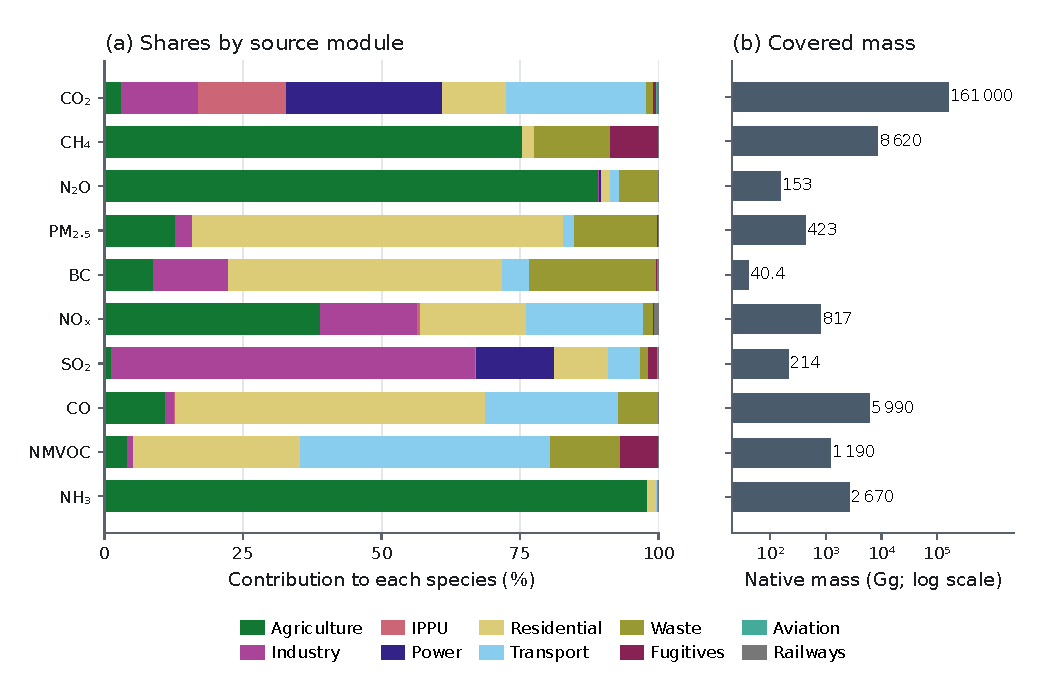
\includegraphics[width=\linewidth]{f09_integrated_composition.pdf}
\caption{Reference source contributions within each species and separate native mass. Shares and absolute quantities answer different questions; the mass axis is logarithmic. Data accompany the figure.}\label{fig:sectors}
\end{figure}

\subsection{Historical change}\label{sec:series}\label{sec:agri-basis}\label{sec:waste-series}
The common panel contains ten fiscal years, July 2015--June 2025. Between FY2015--16 and FY2024--25, covered AR5 GHG changes by \SI{\PakChangeARfive}{\percent}, PM$_{2.5}$ by \SI{\PakChangePMfine}{\percent}, NO$_x$ by \SI{\PakChangeNOx}{\percent}, SO$_2$ by \SI{\PakChangeSOtwo}{\percent} and NH$_3$ by \SI{\PakChangeNHthree}{\percent}. The provisional FY2025--26 source extension is excluded from these endpoints.

Station consumption, sales, crop and nutrient observations supply measured activity changes where available. Census-anchored herd reconstruction, household interpolation/extrapolation and fixed fate parameters supply modelled changes. Coal consumer allocations and edition revisions can cause important industrial changes; a shift in booked kiln fuel is not evidence of a regulatory change in district emissions. Waste history is advanced consistently. Older 1990 calendar diagnostics remain separate and are not spliced onto the common core as uniform fiscal observations.

\begin{figure}[htbp]\centering
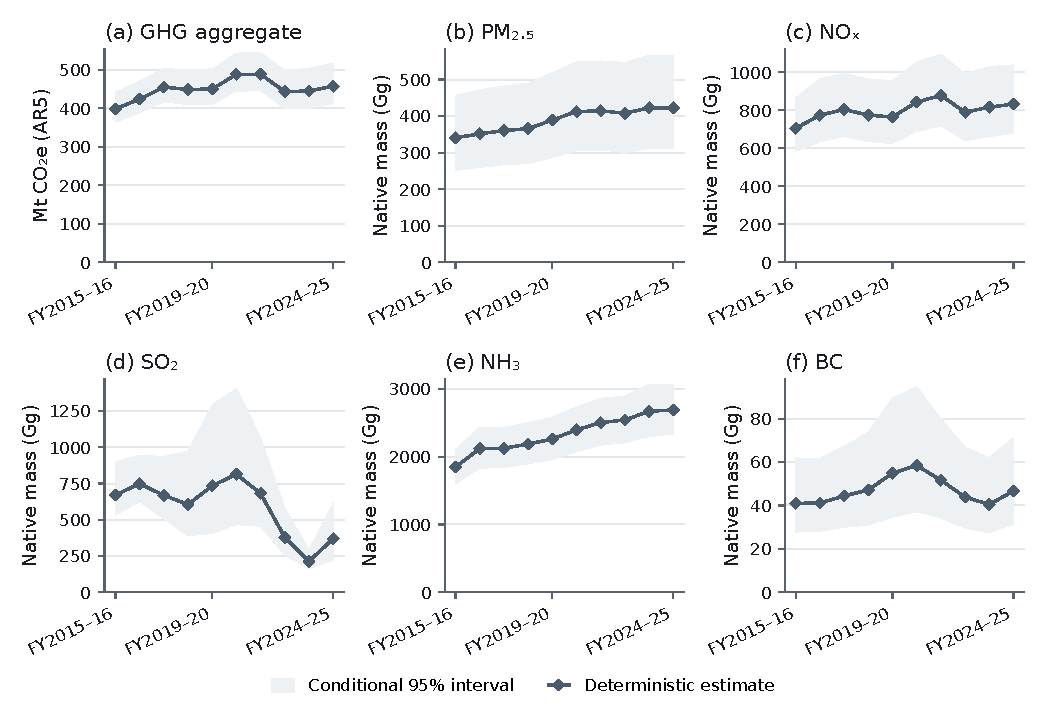
\includegraphics[width=\linewidth]{f10_integrated_trends.pdf}
\caption{Fiscal trends and conditional persistent-parameter intervals. Structural alternatives and missing categories remain outside these intervals. The common core ends in June 2025.}\label{fig:series}
\end{figure}

\subsection{Monthly allocation}\label{sec:monthly}
Annual compatible estimates are allocated through source/process profiles,
\begin{equation}E_{s,p,m}=E_{s,p,t}w_{s,p,m},\qquad\sum_{m\in t}w_{s,p,m}=1.\label{eq:monthly}\end{equation}
Production or sales can be a proxy for emission timing. Fertiliser offtake is supply timing rather than observed application; manure-stage and residue-decomposition release dates are unobserved. Road evaporation and wear do not inherit an observed exhaust fuel profile without evidence. Waste burning, annual flare quantities and unsupported releases retain declared fallbacks. The admitted station subset's aggregate fleet timing is labelled a proxy.

The repaired PBS extraction preserves centred labels, continuation/province rows, source units and worksheet identity. Actual exported province/month values and compatible monthly/annual controls determine admission. Surviving source anomalies are flagged, and national monthly classification requires producing-area completeness; missing observations are not converted to zero. Temporal evidence shares are calculated separately by pollutant.

\subsection{Administrative and grid products}\label{sec:cube}
Source-matched annual weights produce ADM1, ADM2 and 0.05$^\circ$ cell masses under each configuration. Facilities respect commissioning/closure; selected oil/diesel stations use their admitted subset frame, and kiln types retain the supported frame plus an unlocated remainder. Rail geometry excluded from the compatible primary package retains supported administrative mass and explicit fine-scale unallocated mass. Fixed proxies and reference-year patterns retain their evidence class.

\begin{figure}[htbp]\centering
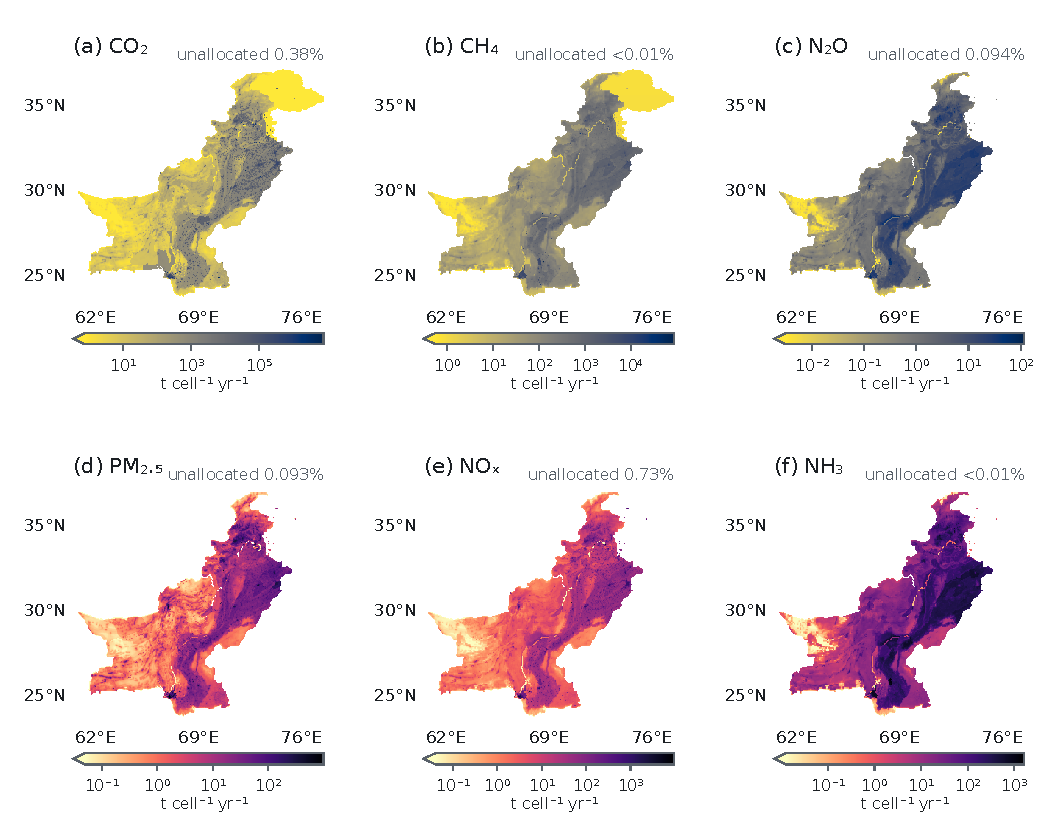
\includegraphics[width=\linewidth]{f11_integrated_maps.pdf}
\caption{Reference native gas and pollutant mass per cell, with separate logarithmic scales. Geographic weights can describe release location, activity origin or accounting; fixed allocation is not observed local change. Unallocated mass is published separately.}\label{fig:maps}
\end{figure}

For each species/configuration/period, annual--monthly and placed--unallocated closure is tested at compatible boundaries. Cell mass is distinct from flux density. Area, country fraction where relevant and duration are required for conversion; vertical injection and detailed chemical speciation remain additional atmospheric-model requirements.

\pkinvEndFragment

\pkinvDemoteFragment
\section{Shared accounting and material constraints}\label{sec:closures}
Shared accounts prevent duplicated source inputs, while explicit residuals retain unresolved evidence. Their numerical closure does not prove the split of material among destinations. Transfers, physical balances and publisher residual identities are different operations.

\subsection{Dung and residue destinations}\label{sec:closure-dung}
Agricultural nitrogen and volatile-solid rates determine diverted dung supply. Reference S receives household survey-supported fuel; material without a supported household destination remains unresolved and is not silently burned. L is the separate all-diverted-household case. The same configuration is applied to GHG, air, monthly, administrative and grid products. Crop residue supply is partitioned among returned soil material, field burning, household fuel and unresolved uses. Household and field combustion are distinct processes and geography.

\subsection{Liquid fuel partitions}\label{sec:closure-generator}\label{sec:closure-offroad}
Household generator petrol and railway diesel are carved out of compatible sales controls before road fuel is estimated. On-road and off-road activity retain their category distinctions. Legitimate records with equal values are not deduplicated by value. Class/fuel/equipment partitions sum to the shared control and are not varied independently as unconstrained uncertainty multipliers.

\subsection{Waste fate}\label{sec:closure-waste}
Collected/disposed, uncollected and burned quantities preserve the supported waste-fate constraints. Disposal CH$_4$ advances the history state rather than using one current year's population as the entire disposal stock. Native uncertainty reruns preserve the material partition and supply the same burned dry mass to air factors. Waste emissions at origin do not establish the physical treatment location.

\subsection{Nitrogen pathways}
Reference TAN follows species/system NH$_3$ losses through housing or yards, storage and field application, acting on surviving total ammoniacal nitrogen. Managed NO$_x$, leaching, N$_2$ and N$_2$O are retained in the common state. Grazing and soil volatilisation remain distinct. The air NH$_3$/NO$_x$ and GHG N$_2$O use the same losses and surviving pools; a separate IPCC configuration regenerates both product families.

Synthetic product factors are kg NH$_3$-N per kg N and receive the 17/14 molecular conversion once. Soil NO$_x$ is calculated on nitrogen and reported as NO$_2$-equivalent using 46/14. The combined volatilised nitrogen used for indirect N$_2$O includes the applicable NH$_3$ and NO$_x$ pathways rather than applying an extra ammonia share to a factor already in NH$_3$-N.

\subsection{Coal and gas boundaries}
The coal account records production, imports, exports/stock information where supported, station power and industrial consumers. Publisher consumer residuals do not establish independently measured use. Unresolved quantities remain explicit; they are not assigned wholesale to kilns. Physical fuel, rank heat and carbon factors remain separate in uncertainty draws. Delivered gas, process feedstock, combustion, leakage, flaring and venting preserve their boundaries without interpreting every flow difference as emissions.

\pkinvEndFragment

\pkinvDemoteFragment
% ===========================================================================
\section{Uncertainty, and What Correlation Does to It}
\label{sec:uncertainty}
% ===========================================================================

Uncertainty is reported three ways: IPCC Approach~1 error propagation per sector, a pooled
Approach~2 Monte-Carlo simulation over every component in the inventory, and the same
simulation run again with the shared emission factors correlated. The third is the one with
a finding in it.

\subsection{Approach 1 and Approach 2 diverge, and the divergence is the finding}

Approach~1 combines each component's relative uncertainty in quadrature, treating correlated
components as summing linearly within their group before the squaring. Approach~2 accumulates
\num{100000} realisations of the national total---and it is a MIXTURE, not one
family: the waste and fugitives modules inject their own sector engines' persisted draws
(waste's ledger-true parameter rerun, whose fate identities hold in every realisation;
fugitives' bounded split-triangular), while every other module draws mean-preserving
lognormals. The draw files, their seeds and their SHA-256 hashes are in the release
manifest and \texttt{outputs/national\_uncertainty\_sources.csv}; the published run uses
ten times the sector default because the paper draws a conclusion from a difference
between two runs, and at \num{10000} draws the reported half-widths carry a Monte Carlo
standard error of the same order as that difference.

The two no longer agree closely, and the gap is the finding: \SI{10.9}{\percent} from
Approach~1 against \SI{11.72}{\percent} from
Approach~2 at the national level---quadrature is the analytic limit of the simulation
only under symmetric, independent, moderate uncertainties, and the injected engines are
deliberately none of those. The honest national statement is asymmetric,
$-\SI{10.3}{\percent}/+\SI{13.1}{\percent}$ about the median
(\texttt{rel\_down\_pct\_95}/\texttt{rel\_up\_pct\_95} in the published table), and a
single $\pm$ figure is printed only as a summary. The interval has two legitimate
reference points and they are not interchangeable: the same 2.5th--97.5th percentile
band (\SIrange{400.30}{504.97}{\mega\tonne}) read against the \emph{deterministic
reference} \SI{444.96}{\mega\tonne} is $-\SI{10.0}{\percent}/+\SI{13.5}{\percent}$,
because the deterministic total sits below the Monte-Carlo median
(\SI{446.52}{\mega\tonne}) and mean (\SI{448.14}{\mega\tonne})---the injected
engines are right-skewed, so re-running the accounting at parameter means does not land
on the distribution's centre. The recommended point estimate is the deterministic
reference \SI{444.96}{\mega\tonne} for accounting and comparison against other
inventories, and the median for any probabilistic statement; a reader attaching the
about-the-median percentages to the deterministic total is off by roughly a point in
each direction, which is why both readings are printed.

\textbf{And this interval is the narrowest statement the release makes, which is the wrong
one to borrow.} It is parametric and annual and national: it prices what the factors and
the activity data could be, and prices nothing about \emph{when} or \emph{where} the mass
was put. Both of those carry their own uncertainty, and neither is probabilistic---a
timing or placement bracket is a disagreement between two defensible readings of the same
evidence, and no probability attaches to a spread. So they are not summed into
$\sigma$. \texttt{outputs/pakemis\_joint\_uncertainty.csv} publishes the three components
separately, per category and per the \emph{resolution of the figure being read}, together
with an envelope---a bound, not a distribution---that widens the parametric interval by the
structural half-widths. A bracket only bites on the figure it can move: re-allocating a
category across districts does not change its national total, and re-profiling it across
months does not change its annual one. Nationally the bound widens from
$-\SI{10.37}{\percent}/+\SI{13.14}{\percent}$ annually to
$-\SI{23.3}{\percent}/+\SI{26.10}{\percent}$ for a district in a month. The four
resolutions form a lattice rather than a chain, because adding a month is not comparable to
adding a district. Timing is priced for seven categories of twenty (six on measured
dispersion, drawn in the ensemble) and placement for six,
and every row names what its envelope therefore omits; filling those cells with a weak
alternative would make the bound look rigorous and be worse.

Within a category the parametric error is perfectly correlated---one emission factor moves
every district and every month of it together---so intervals add \emph{linearly} across
districts and months and never in quadrature, and the gridded products deliberately carry no
per-cell interval that would invite the opposite. Across categories the simulation has
already measured the dependence, and adding the category intervals instead inflates the
national bound to $-\SI{22.0}{\percent}/+\SI{45.3}{\percent}$: not a conservative reading of
the evidence but a different and wrong one, asserting a coupling the correlation model
denies. \texttt{docs/uncertainty\_contract.md} states both rules and
\texttt{tests/test\_joint\_uncertainty.py} proves each by worked example.

\textbf{None of this is validation, and the two are registered separately.} A wide interval
that contains the truth and a narrow one that does not are indistinguishable from inside the
model, so \texttt{outputs/pakemis\_validation\_catalog.csv} records what has been compared
against what: \num{102} entries across the three properties an inventory can get wrong
independently---\num{50} magnitude, \num{20} timing, \num{32} geography---because a national
total agreeing with EDGAR does not validate a map and a satellite hotspot at a facility does
not validate a total. Every entry declares how independent its evidence was, and the answer
is usually not very: \num{20} carry \emph{large} independence, \num{45} only \emph{partial},
and \num{8} \emph{none} at all, meaning the comparison shares the activity data it is
testing (a further \num{10} are by-construction checks to which independence does not
apply). \num{11} rows are declared absences---a module and property with no independent
check, named rather than left blank, because a cell with nothing in it reads as a property
that was never at issue. Six absences in the register this catalogue replaced were found to
be false: the benchmarks had been scoring them all along and nobody had joined the two
registers, so the register understated what the project had actually checked.

Release 1.0.0rc33 unified that register with the frozen benchmark tasks into this one
catalogue (the older register itself was retired in 1.0.0rc35), in which every
validation asset declares its grain, its producer, and how it is wired into the build; a
validation product regenerated by the build itself must now be at least as new as the
build's first output or the build fails naming it, which on first contact exposed one
quality-cited check that nothing in the build produced and one whose producer depends on a
model held outside this repository. The catalogue's verdicts, previously six incompatible
vocabularies, are projected onto one closed set at read time. Its summary,
\texttt{outputs/pakemis\_validation\_scorecard.csv}, tabulates the full property-by-grain
space---magnitude, timing and geography at twelve grains from national to worksheet cell---
and \num{14} of its \num{36} cells are covered today; the remaining cells are written as
declared absences, so the scorecard is simultaneously the record of what has been validated
and the roadmap of what has not.

Three checks added this release each came back \emph{narrower} than they were built to be, and
the narrowing is recorded rather than rounded off. ERA5, on an independent reanalysis, tracks
the NASA POWER temperature behind the residential profile almost exactly in shape---correlation
\num{0.969} to \num{0.989} across five cities and \num{54} months---and disagrees on level by
a systematic \SIrange{3.2}{6.1}{\celsius}. That offset is definitional: the held grid carries
one value per cell per day and no metadata saying which value, so it validates the seasonal
\emph{timing} and cannot validate the degree-day series itself, degree days being a function of
level (\texttt{outputs/era5\_degree\_day\_crosscheck.csv}). APCMA's cement despatches, compiled
by the industry association rather than PBS, reproduce the QIM production shape to a mean
\SI{0.22}{} percentage points of the year over \num{60} months
(\texttt{apcma\_qim\_cement\_crosscheck.csv})---a real corroboration of the shape cement now
rides, on magnitudes that are deliberately not compared because despatches are sales. Its
feedstock corroborates it from a third direction: PBS limestone production tracks the QIM
cement shape to a mean \num{1.20} percentage points of the year over their six overlapping
years (\texttt{limestone\_qim\_cement\_crosscheck.csv}), once one flagged source anomaly is
set aside---November 2016 carries \SI{36.7}{\percent} of its year's limestone in a single
month, a defect in the mines-department series that is published and flagged rather than
dropped. That
parse is gated on three of the publication's own controls---each row's printed total, each
block's annual total, and agreement between the two pages that publish every year---and the
cells failing one are kept unrepaired with their raw text
(\texttt{apcma\_dispatch\_quarantine.csv}, \texttt{apcma\_dispatch\_parse\_summary.csv}). They
include a published digit-grouping error, an annual export total printed as \num{202989} where
its own twelve months sum to \num{2020569}, and small restatements between the two editions of
a year. And FAO's
rice calendar agrees with three of four provincial harvest windows
(\texttt{fao\_crop\_calendar\_crosscheck.csv}), which changed no provenance class, because the
methane profile rides the \emph{flooded} window and harvest is not one of its endpoints.

The divergence localises the assumption doing the work. The completed fugitives ledger gives
$\pm\SI{37.7}{\percent}$ under Approach~1
and $\pm\SI{19.0}{\percent}$ under the injected Approach~2---NARROWER, because the sector
engine's bounded split-triangular draws respect the published range endpoints where the
old lognormal surrogate's tails did not. Its
Monte-Carlo median is \SI{24.15}{\mega\tonne}, its mean
\SI{24.73}{\mega\tonne}---the sector engine's own quantities, reaching the national row
unconverted for the first time.

\subsection{The correlation question}

Six of the ten sector modules report \COtwo{} under an IPCC 1.A code, and they draw it
through the same default carbon-content factors. Transport (both its road and its off-road
categories), electricity generation, industrial fuel combustion, residential fuel, railways
and domestic aviation all take their fuel \COtwo{} factors from the same table entries with
the same published uncertainty ranges. The second case groups those components by the physical
factor each one uses: every row computed with the gas/diesel-oil carbon content draws one
realisation of it, every row computed with the natural-gas content draws another, and the two
are independent of each other. \textbf{It is a declared covariance sensitivity, not an
estimate of the true dependency structure}---see the limitation stated at the end of this
subsection. Process \COtwo{} from cement, fugitive \COtwo{} from venting and flaring,
open-burning \COtwo{} in waste, and agriculture's urea and liming are untouched, because none
of them is fuel combustion.

An earlier edition of this section described a single correlation group spanning all six
modules, which is what the first implementation did. That is not a defensible physical claim:
it asserts that diesel, petrol, natural gas, furnace oil, coal and jet kerosene are all wrong
together, in the same direction, by the same relative amount. It also inflated the correlated
band, and the inflation was most of what the paper had reported as a headline finding.

The membership is derived rather than declared, and that is a repair. Industrial fuel
combustion was outside this group for the whole of the release in which it was added: the
sector list was a hand-written literal that no test compared against the inventory, so a
module burning natural gas and six petroleum products through exactly these table entries was
silently treated as uncorrelated with the rest. The group is now computed from the components'
own IPCC codes---a sector qualifies if it reports \COtwo{} under 1.A---and a test asserts the
declared list equals the derived one, so the next fuel-burning module cannot be omitted the
way this one was.

Treating those draws as independent asserts that the true diesel carbon content could be at
the low end of its range for railways and at the high end for road transport simultaneously.
It cannot. There is one carbon content of the diesel that Pakistan burns, and if the IPCC
default is wrong about it, it is wrong in the same direction everywhere at once.

Almost no published national inventory states which assumption it made. Approach~2 as
described in the Guidelines permits correlation but does not require its declaration, and the
Approach~1 formula makes independence the path of least resistance. We ran both and report
the gap as a result in its own right.

\begin{table}[htbp]
\centering
\small
\begin{tabular}{@{}llrr@{}}
\toprule
& \textbf{Level} & \textbf{Independent} & \textbf{Correlated} \\
\midrule
National mean (Mt \COe{}) & national & 448.14 & 448.15 \\ %
National median           & national & 446.52 & 446.55 \\
2.5th percentile          & national & 400.30 & 400.27 \\
97.5th percentile         & national & 504.97 & 505.22 \\
\textbf{National $\pm$\%} & national & \textbf{11.72} & \textbf{11.75} \\
$-$/$+$\% about median & national & 10.3/13.1 & 10.4/13.1 \\
$-$/$+$\% about det.\ ref. & national & 10.0/13.5 & 10.0/13.5 \\
\midrule
Transport module $\pm$\%  & module   & 12.93 & 12.93 \\
Road transport $\pm$\%    & category & 13.26 & 13.24 \\
Power module $\pm$\%      & module   &  8.34 &  8.34 \\
Residential $\pm$\%       & module   & 30.45 & 30.41 \\
Railways $\pm$\%          & module   & 15.27 & 15.13 \\
Agriculture $\pm$\%       & module   & 21.48 & 21.48 \\
\bottomrule
\end{tabular}
\caption{Monte-Carlo uncertainty (Approach~2, \num{100000} iterations, seed \num{42}), with the
IPCC fuel-carbon factors drawn independently and then with \textbf{one draw per physical
factor}---diesel, motor gasoline, natural gas, residual fuel oil, coal, jet kerosene, other
kerosene and LPG. Every row states its aggregation LEVEL, because the previous edition
reported \num{11.54} in this table and \num{11.96} in the prose beneath it and both were
called ``transport'': one is the module, which includes mixed off-road machinery, and the
other is the road-transport category.
The power module barely moves, and that is a disclosure rather than a null result. Its grid
rows carry the TOE-to-terajoule conversion \emph{and} their fuels' carbon contents as separate
parameters, so they participate in both; what does not move is the balance between them, since
the conversion is shared inside the module under either scope. An earlier implementation gave
each row one group and overwrote this one, which made the
correlated case markedly NARROWER than the independent one---and \emph{positive} shared-factor
dependence should not reduce the variance of the affected non-negative sum relative to
otherwise identical independent draws. That is the form of the claim: correlation in general
can reduce a sum's variance, when it is negative. Every group's draws are anchored to a
representative member row (common random numbers), so the two columns share their randomness
and differ \emph{only} in dependency structure; each remaining movement sits inside three
batch-means standard errors of zero, and the largest anywhere in the table is railways'
0.18 points, where cross-module sharing of the diesel carbon content is a genuine structural
difference. The overwrite was forty.}
\label{tab:correlation}
\end{table}

\begin{figure}[htbp]
\centering
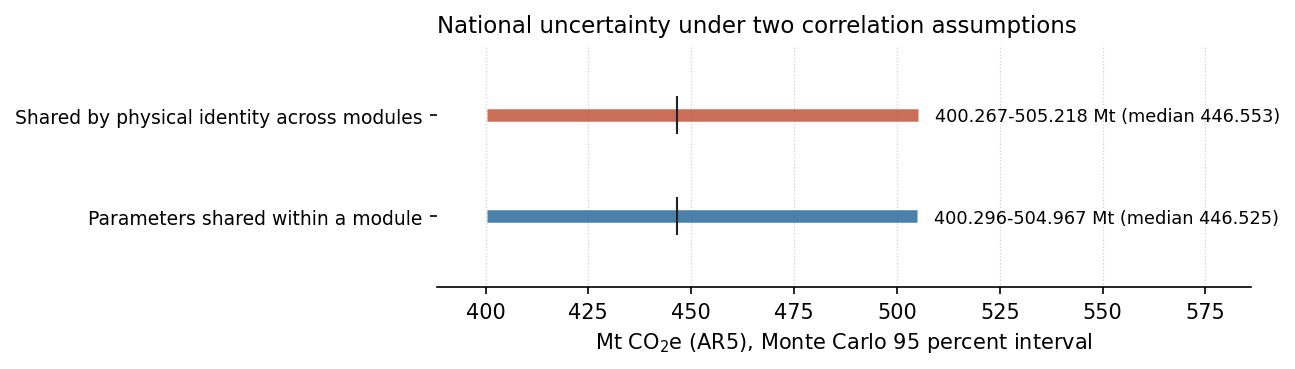
\includegraphics[width=\linewidth]{fig_uncertainty.png}
\caption{95 percent Monte-Carlo intervals for the national total (2.5th to 97.5th
percentile, median ticked) under the two correlation assumptions. The two bars are nearly
identical, which is the finding. Sharing a physical factor prevents the contribution of
that factor from averaging independently across the rows that use it, while preserving each
row's other activity, conversion and residual uncertainties.}
\label{fig:uncertainty}
\end{figure}

\subsection{Reading the gap}

Three things follow, and the first is a correction to what this paper previously reported.

\textbf{At the national level the effect is below the reporting precision:
$\pm\SI{11.72}{\percent}$ either way.} An earlier edition put every fossil-CO\textsubscript{2} component
of every fuel-burning module into ONE correlation group and reported the national band
widening by a fifth. That grouping is not a physical claim. It asserts that the IPCC carbon
contents for diesel, petrol, natural gas, coal, furnace oil and jet kerosene are all wrong
together, in the same direction, by the same relative amount. Grouped per factor---which is
what the shared-default argument actually supports---the eight factor groups are independent
of one another, their variances add in quadrature, and the national effect largely cancels.
The finding as previously stated was an artefact of the grouping.

One coupling was, however, genuinely missing rather than over-asserted, and closing it
is what brought the two scenarios onto the same reported figure. Urea \COtwo{} is
\emph{derived} from the audited national nitrogen offtake---the same series that drives
the synthetic-fertiliser soil pathways---yet the scope registry named that one series
twice, once per receiving category, so a draw moved managed soils and urea application
independently. No physical reading supports that: if the national offtake is wrong, it
is wrong for both. Scoping it as one parameter across both categories is that change, and it widens the
agriculture band by about a hundredth of a percentage point---the direction the
supplement predicted, at a magnitude far below what any reader should act on.

\textbf{At parameter level the effect becomes negligible and is indistinguishable from
Monte Carlo sampling noise at the reported precision.} The
transport module reads $\pm\SI{12.93}{\percent}$ under both correlation structures and the
road-transport category from $\pm\SI{13.26}{\percent}$ to $\pm\SI{13.24}{\percent}$---a
movement smaller than the batch-means standard error published beside its band. The earlier edition reported the road
category widening from \SI{11.96}{} to \SI{18.46}{\percent} on this assumption, and that was
an artefact of the model rather than a property of the inventory: a component could carry only
ONE correlation group, so putting a row in the fuel-carbon group made its \emph{entire}
variance move with the factor. The carbon content of diesel carries about \SI{2}{\percent};
a road class row carries thirty to sixty. Correlating two points of a fifty-point variance
across rows cannot widen their sum, and once the row's activity, conversion and factor are
carried separately it does not.

\emph{The road-transport band is wider than the previous edition published}---\SI{13.3}{}
against \SI{12.0}{\percent}---and that is the same correction seen from the other side. The
OCAC Road control is genuinely one quantity behind every class row, and the old model had no
way to say so while the fuel factor occupied the row's only correlation slot.

\textbf{Once uncertainty is decomposed by parameter, cross-module sharing of the same
physical fuel-carbon factors has a negligible effect on both national and transport
intervals.} The earlier large effect was created by moving the whole component variance with
a factor representing only a small portion of that variance. The argument for publishing the
correlation model beside every band survives the correction: the two scenarios answer
different questions, and only reporting both shows that the answer no longer depends on
which one is asked.

The correlated case is a \emph{bound}, not a better estimate. Perfect correlation is as
strong an assumption as perfect independence, and the truth is between them: the six modules
do share an IPCC default, but they burn physically different fuel batches with genuinely
different carbon contents, and their activity uncertainties remain independent. We report
both endpoints and choose neither, on the same principle applied to the waste sector's
disputed methane correction factor. The honest statement is that the national uncertainty is
$-\SI{10.3}{\percent}/+\SI{13.1}{\percent}$ about the median (symmetric summary
\SI{11.8}{\percent}; $-\SI{10.0}{\percent}/+\SI{13.5}{\percent}$ about the
deterministic reference) under either assumption, and that what the assumption is worth at
national scale is now smaller than the Monte Carlo noise on the estimate.

\textbf{What this exercise is, and what it is not.} It is a \emph{declared covariance
sensitivity}: two named dependency assumptions, run and reported, with the difference between
them attributable to the assumption. It is not an estimate of the true covariance structure of
the underlying activities and factors, and it should not be read as a confidence bound on that
structure.

What the two scenarios vary is \emph{where sharing stops}. A component's draw is the product
of one multiplier per named parameter that enters it and a residual multiplier private to the
row, so a power gas row draws the TOE-to-terajoule conversion, the IPCC carbon content of
natural gas and its own metered activity as three separate quantities. Under the
within-module scope every parameter is qualified by its module, so the carbon content of
diesel is treated as a different quantity in railways and in road transport---which is what an
inventory compiled sector by sector implicitly assumes. Under the cross-module scope it is one
quantity everywhere.

An earlier edition of this machinery gave each component a single correlation group. That
forced a choice between a row's conversion and its factor, and excluded the power module from
the fuel-carbon scenario altogether because its rows were already spoken for by the TOE group.
That limitation is gone. The one that remains is coverage rather than architecture: a
parameter can be shared only once it has been named, and the registry does not yet name every
quantity behind every row. Section~\ref{sec:paramcoverage} reports how far it reaches.

\subsection{Parameter coverage, and what the variance is attributed to}
\label{sec:paramcoverage}

Sharing parameters requires naming them, so the natural question is how much of the inventory
the registry reaches. The answer should be read as a statement about the registry rather than
about the physics.

Of the \num{202} component rows, \num{202} carry at least one named parameter and \num{200}
carry more than one---the case the previous machinery could not express at all. The registry
holds \num{672} parameters; \num{141} dependency groups carry variance in the published run,
and 92 of those enter more than one row, which is what makes correlation possible at
all. The largest single addition is agriculture's factor table
(\texttt{outputs/agriculture\_uncertainty\_inputs\_2024.csv}): the sector composed its IPCC
factor uncertainties inside each row's declared width, where the registry could not see
them, and naming them---the same values, the same widths, no new numbers---is what
brought them inside it. Each row's marginal is decomposed as a sum over its named parameters plus a residual:
where the declared row width covers its parameters, the residual closes the identity exactly
and the marginal is the declared one; where the named parameters imply \emph{more} variance
than the row declares, the parameter graph is authoritative---the marginal is derived from
the parameters under a per-row disposition in
\texttt{data/uncertainty\_reconciliation.csv}, and the declared width is published beside it
as a comparator. The audit register carries \num{59} dispositioned rows: the original
twenty-three were rows a previous edition clamped silently, and the audit found most of
them one resolver defect (a median summarising a multi-member group with another row's
width); after its repair \num{37} rows remain derived at the reference year, each carrying
a named cause---a declared width that omits terms the sector's own input table carries, or
a sector width propagated through a nonlinear model the linear quadrature legitimately
disagrees with. Seven of the dispositions are the naming's own find: HISTORICAL panel
years compose the FAOSTAT projection's activity widths while the registry holds the census
year's, so those rows derive from the graph in the panel years and reconcile exactly at
the reference---the vintage difference published, not clamped. The twelve newest are the
manure and managed-soils N$_2$O rows: once the herd and crop draws were scoped to the
streams they physically drive, their declared widths---the emission factor's alone---were
found to omit the activity the engine multiplies in, and the graph now carries them at
\SIrange{107}{124}{\percent} against the \SIrange{101}{114}{\percent} they declared.

Which quantities drive the national uncertainty is read from the released ensemble itself,
not from a decomposition fitted to it. \texttt{outputs/pakemis\_uncertainty\_drivers.csv}
gives each category's and each module's share of the variance of the national total across
the \num{10000} released draws---the covariance of the category with the total over the
variance of the total, so the shares sum to one---its share of the excess in the top and
bottom 2.5 per cent of draws, and the national interval with that one category held at its
deterministic value. Enteric fermentation carries \SI{59.8}{\percent} of the variance,
managed soils \SI{14.0}{\percent}, domestic wastewater \SI{9.0}{\percent}, manure
management \SI{5.6}{\percent} and rice cultivation \SI{4.0}{\percent}; by module,
agriculture carries \SI{83.5}{\percent} and waste \SI{11.1}{\percent}. The upper tail has
the same order: of the excess in the top 2.5 per cent of draws, enteric fermentation is
\SI{60.1}{\percent}, managed soils \SI{14.7}{\percent} and domestic wastewater
\SI{10.5}{\percent}. With enteric fermentation held fixed the national interval narrows
from \SIrange{399.8}{505.4}{\mega\tonne} to \SIrange{420.3}{483.9}{\mega\tonne}.

The product carries one parameter row. The wastewater effluent factor, frozen at its
default in a rerun of the waste engine on the same draws, carries \SI{4.1}{\percent} of the
national variance and \SI{4.8}{\percent} of the upper tail. Parameter-level importance is
not otherwise claimed. Earlier editions ranked named parameters by Sobol indices estimated
on a surrogate of the simulation; that decomposition, its estimator sweep and its
convergence table are retired, with every figure drawn from them.

\subsection{What the interval leaves out}
\label{sec:bridge}

The interval above is \emph{conditional on one structural configuration}, and that
configuration is larger than any one axis of it. The residential dung basis is a single
axis---which reading of the dung evidence the residential sector takes, the household survey in the reference---while the
\SI{444.96}{\mega\tonne} total rests on \num{23} such choices, of which it is one. Configuration~L, the alternative on that axis, is a first-class key rather than a delta: the annual product carries its residential rows under \texttt{configuration\_id}, beside the reference's typed dung residual, its spatial products are gridded through the same dispatch as the reference: \texttt{pakemis\_grid\_0p05\_monthly\_ledger.nc}, \texttt{pakemis\_adm1\_ledger\_2024.csv} and \texttt{pakemis\_adm2\_ledger\_2024.csv} at stream~$\times$~gas~$\times$~month, differing from the reference in the two dung-cake streams' masses and in no other cell, and \texttt{pakemis\_ensemble\_ledger\_summary.csv} prices it on the same \texttt{draw\_id} as the reference ensemble, so the configuration delta is a per-draw difference rather than two unrelated intervals. They are recorded as a scenario
registry, \texttt{REF\_2023\_24} in \texttt{data/scenarios.csv}, and the release manifest
carries the whole object rather than the letter.

Figure~\ref{fig:bridge} prices each published alternative and draws the one unpriced axis as a labelled empty slot; \texttt{outputs/national\_axis\_register.csv} is the definitive one-row-per-axis table (family, reference setting, deltas, pricing status, and the reason where unpriced). The coal energy basis in
power is worth \SI{1.6}{\mega\tonne}, the sewer methane correction factor
\SI{9.1}{\mega\tonne}, and the fugitive practice assumption \SI{8.6}{\mega\tonne}. Each of
those is \emph{smaller} than the parametric interval, which is about \SI{52}{\mega\tonne} at
the 95th percentile---and \emph{none of them is inside it}. That is the point, and it is not
the same point as being larger: the interval is conditional on the reference configuration and
does not vary these axes at all, so their effect is not represented in it at any width. A
reader given only $\pm\SI{11.7}{\percent}$ has no way to see that they exist.

\begin{figure}[htbp]
\centering
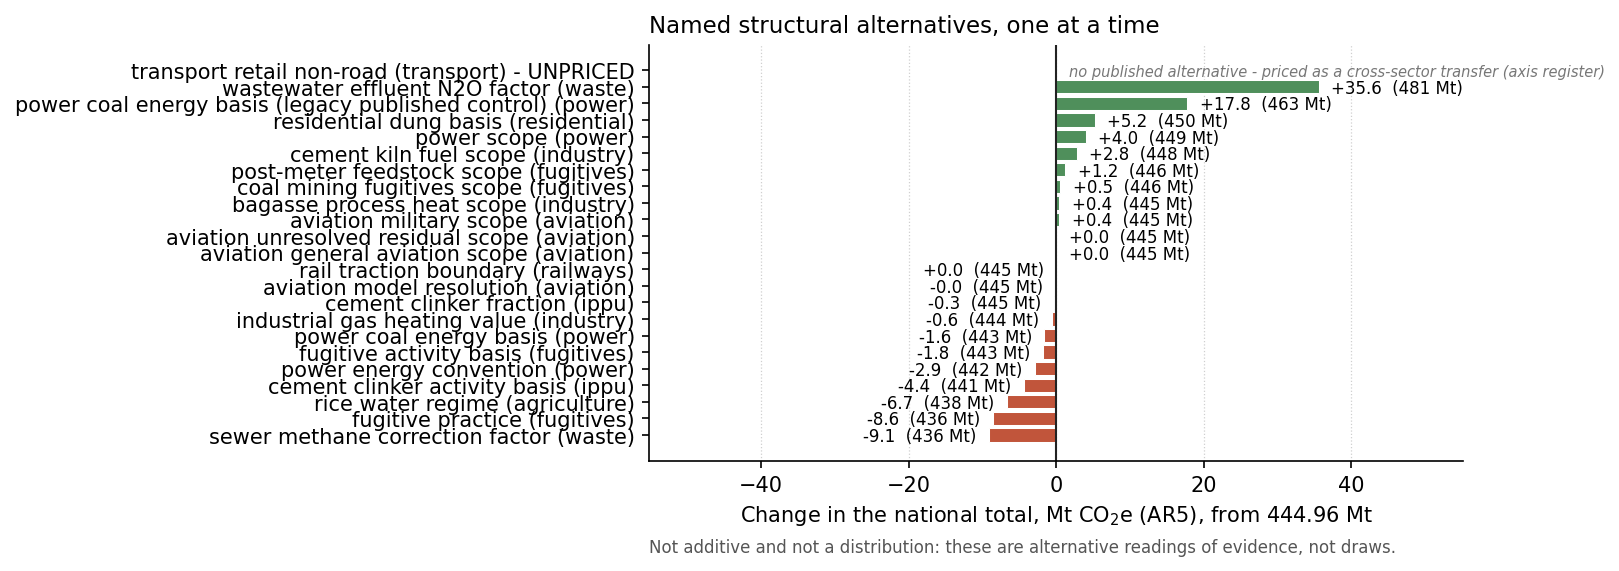
\includegraphics[width=\linewidth]{national_structural_bridge.png}
\caption{The deterministic effect of each named structural alternative on the national total,
one at a time, from \texttt{outputs/national\_structural\_bridge.csv}. \textbf{The bars are not
additive and are not a distribution.} Two of the power axes describe the same coal energy in
different ways and cannot both be taken; none carries a probability, because assigning one
would be the fiat this inventory declines. The transport retail non-road axis has no
single published alternative and is priced as a cross-sector
transfer in the transport supplement instead.}
\label{fig:bridge}
\end{figure}

The same pricing ships in a second, policy-facing form:
\texttt{outputs/national\_configurations.csv} names nineteen single-axis
configurations---the reference, seventeen alternatives a policy reader would ask for by
name (the aviation scope fork ships as three of them: military
attribution, general-aviation activity and the bridge's unresolved residual are
separate evidence questions, priced separately; the post-meter feedstock scope returns
fertilizer feedstock to the leak base, the membership of every release through rc66, retained
and not defended, and the newest is the power coal
calorific basis, which asks the coal-energy question a second way with no heat
rate anywhere in it and so, unlike the member beside it, does not divide the
generation back out of an energy that contains it), and one reporting recode whose
delta is zero by construction---each the scenario
with exactly one axis moved to its published alternative
reading, resolved through the same machinery as the bridge so the two products cannot
disagree. Eight further rows are declared exceptions to the one-axis rule, each
labelled as the exception it is: the fugitives envelope floor (seven axes at their
minimal legs at once), the cross-sector gas deduction (a net-of-leakage adjustment
no single module's scenario table can carry), the central practice reading
(a third reading of the fugitive-practice control, which the one-alternative-per-axis
registry schema cannot hold), and the five scope screenings whose categories sit
outside every module's own scenario table---the F-gas consumption bound, the
commercial/institutional floor, nitric acid unabated and at its last verified
abatement, and the ammonia gas-balance ceiling. The reference now books the stations' own metered coal at IPCC rank defaults, so the
members of this family describe the accounts it replaced. If the coal energy is instead
taken at the calorific values the plants' own generation implies---the heat-rate route,
whose energy contains the generation it is later divided by---the total is
\SI{443.4}{\mega\tonne} (\emph{power\_plant\_physical\_coal}); on NEPRA Table 3's
published conversion, the reference for every release before the coal re-base and retained
as a named control because it implies net fleet efficiencies outside 28--47 per cent in
seven of nine years---it is \SI{462.7}{\mega\tonne}
(\emph{power\_table3\_legacy\_control}); if the Tier~1
clinker model at the 0.75 fraction were taken in place of the producer census, it is
\SI{440.5}{\mega\tonne} (\emph{cement\_tier1\_model\_low}); with the K-Electric system's fuel added to
the power boundary it is \SI{449.0}{\mega\tonne} (\emph{power\_with\_kelectric}), a coverage
alternative priced beside the reference and not added to it: whether the national fuel
statistic already contains K-Electric's fuel is not established, and if it does, adding it
would count that fuel twice.

The file also carries a structural grouping: the power alternatives and the reference are
labelled ONE FAMILY (\texttt{family\_id} \texttt{power\_grid\_control}), because they are
competing definitions of the same grid control---38.45, 40.04, 44.05 and
\SI{57.82}{\mega\tonne} at the sector level---rather than independent axes. They are not
alternatives of one kind, and the file's \texttt{family\_kind} column says which each is:
38.45 is a fuel-property alternative on the reference's own fleet, 44.05 a coverage
alternative that adds the K-Electric system's fuel, and 57.82 a legacy published account
retained for traceability. A range may be formed only within one kind.

\textbf{The selection rule changed with this release, and the previous one rested on an
argument that does not hold.} Every release until now took the regulator's published
national statistic, and the declared reason was that Pakistan's UNFCCC filing agreed with
it on solid fuels to 2\,per cent, which was held to be standing counter-evidence against
the plant-implied coal case. That agreement is not evidence: the filing is compiled from the
same energy balance the regulator reports, so the two agree by provenance, and
\texttt{data/validation\_catalog.csv} has carried that row at independence class
\texttt{none} throughout. The rule now rests on a test neither account can satisfy by
construction. Dividing each candidate coal energy into the regulator's own printed
generation gives an implied net fleet efficiency; against the 28--47\,per cent envelope the
published conversion lands inside in TWO of nine panel years and the generating stations'
own metered coal at IPCC rank default calorific values lands inside in SEVEN, with the
remaining two straddling the envelope rather than falling outside it. Those two are
FY2016--17 and FY2017--18, the years whose commissioning coal is bounded rather than
printed, and the straddle is a property of that interval: it is bounded by the intensity
range the same two stations run at over the ledger years, which includes a sharply
curtailed year, and a commissioning plant is a part-load plant, so the low-intensity end
of that range is the relevant one rather than an outlier to discard. A narrower band
would place the whole interval inside the envelope, and would do so by excluding the most
analogous observation available. Neither side
of that test touches a heat rate, so neither restates the regulator's own print---which the
third candidate, the heat-rate route at \SI{38.45}{\mega\tonne}, does by construction and is
why the re-base did not go there.

The reference is therefore \SI{40.04}{\mega\tonne}, and the conversion it replaced is
retained as \texttt{power\_table3\_legacy\_control} at \SI{57.82}{\mega\tonne} rather than
deleted, so a reader holding a total published before this release can find the account it
came from. It is not equally probable with the reference and the registry says so, which is
also why it is excluded from the priority ranking of unresolved choices. The per-year moves,
and the mass and calorific terms whose product is each year's ratio, are published in
\texttt{outputs/pakemis\_power\_coal\_rebase\_ledger.csv}; the four candidate accounts with
their efficiency verdicts are in
\texttt{outputs/pakemis\_power\_coal\_configurations.csv}. Every quote of the grid figure,
here and in the results section, is conditional on that rule with the alternatives named
beside it; the structural bridge carries the same \texttt{family\_id} tag on its power axes.

One constraint on those candidate explanations is new here and narrows all of them at
once. Each supposes a constant difference between the regulator's two tables---a calorific
convention, a gross basis, a scope, a stock change---and a constant difference has a
constant sign. Across the five years the plant ledger spans it does not.
\texttt{outputs/pakemis\_power\_coal\_energy\_adjudication.csv} divides each energy
figure by the coal generation the regulator itself reports, a test that uses no tonnage and
so cannot be undone by an error in one: Table~3's energy implies a fleet net thermal
efficiency of \SI{57.5}{\percent} in FY2020--21 and \SI{18.9}{\percent} in FY2023--24.
No thermal fleet spans that range, and a plant set that is too wide makes energy too high
in every year rather than too low in one. Over the same years the plant-level route implies
\SIrange{32.4}{45.7}{\percent}, which is a fleet.

The break is dated, and it is not a revision between editions: the 2024 edition prints
FY2018--19 to FY2021--22 side by side in the same table, and the 2025 edition reproduces
those columns exactly. Across two adjacent columns of that one table the coal
tonne-of-oil-equivalent figure rises \SI{87.5}{\percent}, from \num{4123008} to
\num{7731514}~TOE, while the same report's per-station table has coal mass falling
\SI{7.3}{\percent} and coal generation falling \SI{3.5}{\percent}.

It \emph{is} a conversion, and over a panel longer than the plant ledger it is a constant
one. Table~3 states that it takes these figures from the HDIP \emph{Pakistan Energy
Yearbook}, and HDIP's own power-sector coal tonnage is held here as well, republished in the
Economic Survey's statistical supplement. Against \emph{that} tonnage Table~3's energy works
out at \num{0.447} tonnes of oil equivalent per tonne in every year from FY2015--16 to
FY2020--21---six consecutive years spanning \num{0.000072}~TOE per tonne, or
\SI{0.016}{\percent}---and \num{0.604}, \num{0.511}, \num{0.478} thereafter.
\texttt{outputs/pakemis\_power\_reference\_audit.csv} carries the span year by year, and
\texttt{outputs/pakemis\_power\_fuel\_reconciliation.csv} carries the plant, fuel and year
account the constant is measured against: coal mass, rank, generation and the energy they
imply, for all nine years rather than the five the per-station table reaches, with the
edition and table each number was read from and an interval wherever no edition prints a
mass. That
constant is \SI{18.73}{\tera\joule\per\giga\gram}: one generic coal factor, applied whatever
the fleet happened to be burning. It breaks in FY2021--22, and it breaks \emph{upward}---to
\SI{25.27}{}, then \SI{21.40}{} and \SI{20.02}{}---over exactly the years the fleet's own
physical calorific value falls from \SI{20.34}{} to \SI{13.01}{\tera\joule\per\giga\gram} as
Thar lignite scales. A measured energy cannot move the wrong way against its own fuel. An
earlier version of this section read the first two of those six years and concluded the
opposite; the panel simply began too late to see the constant. What \emph{also} moves is the
ratio of the two tonnage accounts: HDIP's national series against the regulator's own per-station
quantities runs \num{0.88}, \num{0.70}, \num{1.05}, \num{1.11}, \num{1.21}, crossing unity
between the two years in question. A scope difference cannot cross unity. A
consumption-against-receipts difference could, in either direction, and nothing held settles
which.

A physical screen then narrows them, though it does not choose between them. Taking each
tonnage account at the fleet's own rank composition---IPCC default calorific values, no heat
rates---and dividing the electricity out of it, the per-station account gives
\SIrange{34.4}{38.7}{\percent} in every one of the five years: a fleet, inside the band
throughout. HDIP's national series gives \SI{49.0}{\percent} falling to \SI{29.1}{\percent},
outside at both ends. Of three accounts of the same coal, one is physically admissible across
the panel and two are not. That screen is a plausibility filter on a candidate energy level
and \emph{not} independent corroboration of the account it favours: the efficiency it reports
is the electricity divided by exactly the energy that route constructs, which is an identity
rather than a comparison, and the audit above recomputes it year by year to show so. It can
reject an energy level as unphysical; it cannot adjudicate between two tonnage accounts that
imply the same energy.

\texttt{outputs/pakemis\_power\_coal\_configurations.csv} states the four candidate coal
accounts year by year with what each depends on, and the column that matters is whether the
calorific value was derived from generation. One of them was: the \SI{38.45}{\mega\tonne}
alternative this paper names beside the reference takes heat-rate-implied calorific values,
so its energy contains the generation it is later divided by and its implied efficiency
restates the regulator's own print rather than testing it. The rank-default route, which
uses no heat rate and is the only candidate independent of the electricity it is judged
against, was published nowhere before that file. Its ratio to the published energy runs from
\num{0.47} to \num{2.00} across the panel and crosses unity twice, and decomposes exactly
into a tonnage term that stays within \numrange{0.74}{0.99} and a calorific term that runs
\numrange{0.63}{1.38}: the sign change is the conversion, which is why no single correction
factor exists. That the composition is
genuinely moving underneath all three is not in doubt: the fleet's lignite share by mass goes
from \SI{27.6}{\percent} in FY2020--21 to \SI{39.3}{\percent} in FY2021--22 and reaches
\SI{92.0}{\percent} by the reference year, which is why a calorific value that rises over
the same span is the wrong shape whatever tonnage it is divided by. A third route, taking the
same tonnages by rank at IPCC default calorific values and no heat rate at all, falls with
the fleet as the plant route does.

None of this overturns the selection. The official reporting filing agrees with the
regulator's coal energy to within \SI{2}{\percent}, which is the standing counter-evidence
the rule already cites, and this inventory continues to take the published national
statistic. What the constraint establishes is narrower and, for a reader deciding how much
weight the \SI{40.04}{\mega\tonne} figure carries---against the \num{38.45},
\num{44.05} and \num{57.82} alternatives named beside it throughout---more useful: whichever reading is
right, it is not one that holds constant across the panel, so the open question is not only
\emph{which} table to believe but \emph{when} its basis changed.
No probability attaches to any row---the schema forbids the column---and the rows do
not compose: each is one axis off the reference, not a corner of a scenario space.

One axis carries a finer question than its name, and it gets its own table. Under
the reference the household survey observes \SI{10.93}{\mega\tonne} of dung cake against
the ledger's \SI{58.74}{\mega\tonne} diversion, and mass conservation cannot say where the
other \SI{47.81}{\mega\tonne} went---conservation proves the mass exists, not its
destination. But the candidate destinations are not interchangeable: each has different
\CHfour{}, \NtwoO{} and biogenic-\COtwo{} consequences, so the survey reading alone under-describes the
national reading. Table~\ref{tab:dungvariants} prices each destination declared in
\texttt{data/scenario\_variants.csv}, with no probabilities. The non-household-combustion
variant lands on the L~total exactly, because the residual burning anywhere on the same
fuel chain emits what L counts---a reclassification, not a new quantity---and that
equality is asserted by test rather than observed. The survey reading carries its own
uncertainty, and the reference prices it: the dung stream is drawn at \SI{35}{\percent}
activity uncertainty, the width firewood carries.

\begin{table}[htbp]
\centering
\footnotesize
\begin{tabular}{@{}p{0.46\linewidth}rr@{}}
\toprule
\textbf{Destination of the 47.81 Mt residual} & \textbf{$\Delta$ vs reference} & \textbf{National} \\
\midrule
Declared unresolved stock (the reference) &  0.00 & 444.96 \\
Non-household combustion, same fuel chain & 5.25 & 450.20 \\
Return to manure management               & 4.49 & 449.44 \\
Field application (soils \NtwoO{})        & 3.49 & 448.44 \\
Diversion fraction revised down           & 4.49 & 449.44 \\
\bottomrule
\end{tabular}
\caption{National consequences of each destination for the reference's unresolved dung
residual, Mt \COe{} (AR5), from \texttt{outputs/national\_dung\_variants.csv}. Every
variant conserves the diverted mass exactly (asserted at write time); none carries a
probability. Return-to-manure and revised-diversion price identically because the
arithmetic is the same---what differs is which reading of the evidence is being revised,
and the published note says so. The residual is worth between \num{3.5} and
\SI{5.2}{\mega\tonne} depending on where it went, which is why conservation alone cannot
close the scenario.}
\label{tab:dungvariants}
\end{table}

\subsection{One ensemble, joinable: the common draw\_id}
\label{sec:ensemble}

Until this release, every uncertainty product answered its own question in its own file
and nothing shared a draw: the annual Monte Carlo published percentiles, the monthly
layer carried deterministic brackets, the spatial products carried none by declared
design. A reader could not ask ``in the realisations where the national total is high,
which months and which provinces are high?''---and the two closure identities the
deterministic products enforce at $10^{-9}$ were not even \emph{expressible} per draw.
The common ensemble makes them expressible and then asserts them inside every one of its
\num{10000} draws: \texttt{outputs/mc\_draws/pakemis\_ensemble\_\{annual,monthly,%
spatial\}.parquet}, joined by a single \texttt{draw\_id}, with
$\sum_{m=1}^{12} E(d,c,m) = E_{\mathrm{annual}}(d,c)$ and
$\sum_{\mathrm{prov}} E(d,c,p) + E_{\mathrm{retained}}(d,c) = E_{\mathrm{annual}}(d,c)$
holding to $10^{-9}$ in every draw $d$ (the second is the gridded-plus-unallocated
identity, carried as a placement axis). Every stream in the national pool is
identity-seeded, so draw $d$ of the ensemble is \emph{bit-identically} draw $d$ of the
published \num{100000}-draw run---a prefix given a name, not a second simulation---and a
test asserts the bit-identity. The summary surface
(\texttt{outputs/pakemis\_ensemble\_summary.csv}) publishes each grain's quantiles with
batch standard errors beside the published run's, which is the convergence statement for
the prefix.

What is drawn and what is not follows the evidence, per category and stated in a column.
Monthly profile weights are \emph{drawn} only where a measured dispersion exists---the
hindcast WAPE streams, road transport and railways, whose weights take multiplicative
noise sized by the measured error and renormalise to sum to one inside every draw---and
are degenerate everywhere else
(\texttt{profile\_uncertainty\_status}); the power fuel-mix variant remains a conditional
configuration and is never mixed in. Spatial shares are fixed per draw---allocation is
declared, not sampled---so the spatial layer's per-draw variation is the parametric mass
reaching each province, and the priced allocation alternatives ship as conditional
quantile blocks over the same draw\_ids
(\texttt{outputs/pakemis\_ensemble\_spatial\_conditionals.csv}), never as a mixture. A
month-by-cell ensemble would be roughly \num{118} gigabytes and is deliberately absent:
the ensemble is marginal by design, category grain for months and province grain for
space, and the deterministic weights whose sums-to-one the cube gates already enforce
carry each draw the rest of the way. The five kinds of uncertainty this release
separates---parameter, profile, placement, structure, completeness---each have a carrier
product and an aggregation rule, stated in \texttt{docs/uncertainty\_contract.md}; the
completeness kind rides the joint lattice as a bound
(\texttt{completeness\_bound\_Mt}) beside the interval, never a distribution inside it.

Structure gains a time axis the same honest way. The twenty-two registered axes were priced
against the reference year only;
\texttt{outputs/pakemis\_structural\_trajectories.csv} now re-prices each axis in each of
the nine panel years where its engine honestly can---92 axis-years priced on their
own years' activity---and refuses the rest with the missing evidence named per row
(93 refusals; the producer
census that is own-year by construction, the scenario runners that price the reference
year only). A refusal is a row, never a silence, and no probability attaches to any
point: these are deterministic forks re-read per year, not a trajectory ensemble, and the
longitudinal product's refusal to cross structural axes into a probabilistic ensemble
stands.

\subsection{Where the uncertainty actually lives}

The national band is much narrower than most of its sectors'---\SI{10.9}{\percent} against
waste's \SI{51.1}{\percent} and fugitives' \SI{37.7}{\percent}---which is the ordinary
behaviour of partly independent errors in a sum. Fugitives now contribute
\SI{5.3}{\percent} of emissions and \SI{3.3}{\percent} of Approach-1 variance. Its discrete
practice and coverage scenarios remain outside the pooled Monte Carlo, so the national
probability interval should not be read as absorbing that structural envelope.

The same caveat now applies to electricity generation, whose uncertainty was rebuilt
around its evidence classes: its parametric band fell to $\pm\SI{8.3}{\percent}$ (per-fuel
activity widths, correlated through the shared TOE conversion) precisely because its
one-sided questions---the coal calorific conversion (worth \SI{1.6}{\mega\tonne}), the
TOE gross/net basis, and K-Electric coverage---moved into named structural cases with
conditional intervals and no probabilities. The national interval absorbs none of them,
and the power sector's scenario table is where a reader finds what they are worth.

\subsection{What to measure next depends on the question}
\label{sec:priorities}

The driver shares above answer one of three different priority questions this inventory
publishes, and they are not
interchangeable. Which \emph{category} would most narrow the conditional interval is
a parametric question, and its answer is enteric fermentation, read from the ensemble at
category grain with no ranking of named parameters. The other two are published together
(\texttt{outputs/national\_priority\_rankings.csv}). Which \emph{unresolved model
choice} most moves the deterministic total is a structural question the interval cannot
see, and its answer is the power coal energy basis at \SI{9.1}{\mega\tonne}. Which
\emph{missing category} most changes completeness is a coverage question neither of the
first two can express, and its answer is industrial solid fuel:
EDGAR carries \SI{19.4}{\mega\tonne} for 1.A.2 that this inventory does not estimate.
Reading any one of the three as the measurement priority list silently answers the other
two questions with it.

\subsection{Nine years, and whether their differences are resolved}
\label{sec:longitudinal}

Everything above conditions on the reference year. The nine-year panel is the product a
reader is most likely to difference, and until now it carried no interval at all---so the
only bound available for a year-on-year change was the national
\SIrange{-10.4}{16.0}{\percent}, which is a statement about a \emph{level} and does not
apply to a \emph{change}. \texttt{outputs/pakemis\_longitudinal\_uncertainty.csv} gives every
fiscal year a band and \texttt{outputs/pakemis\_trend\_uncertainty.csv} gives every
consecutive pair and the full window one, differenced draw by draw so that shared error
cancels as the real quantity does.

How much of it cancels is not something the evidence settles, so three correlation scenarios
are published rather than one. At one extreme every component's error is a single draw shared
by all nine years; at the other every error is redrawn wherever the underlying number moved.
The reported scenario is neither: it is typed from the parameter graph, sharing across years
what names a factor, a physical constant or a held parameter, and redrawing what names a
quantity measured in a particular year. Whether a quantity ``moved'' is decided by equality
in-process and enters a stream's seed as the first fiscal year that carries the value, never
as the value's own digits: a one-ulp platform difference in a computed number therefore cannot
re-seed a stream, and the first \num{200} draws of every stream ship as
\texttt{outputs/pakemis\_longitudinal\_prefix.csv} so that a rerun elsewhere is compared with
what this release drew rather than trusted.

\textbf{The resolution statement, read from the product's own rows with scenario and
scope named on every number.} Under the reported (typed) scenario, \num{2} of the \num{8}
consecutive year-on-year changes in the panel are resolved at \SI{95}{\percent}. The
decadal window IS: since the FY2015--16 recovery the panel has one window rather than
two---the common-scope span and the full panel coincide at ten comparable sectors---and
the FY2015--16 to FY2023--24 change of \SI{51.12}{\mega\tonne} resolves at
\SIrange{15.94}{89.57}{\mega\tonne} under the typed scenario and at
\SIrange{40.08}{64.04}{\mega\tonne} under time correlation, but NOT under the
deliberately-widest reading, full time independence
(\SIrange{-10.01}{114.07}{\mega\tonne}), which spans zero.

\textbf{That is a retreat from what this paragraph said before the coal re-base, and the
retreat is the honest reading.} It said that no end of the bracket left the decadal change
spanning zero any more. That was true of the larger change the previous edition
reported and is false of this one under the same intervals. Booking public-power coal on the
generating stations' own metered fuel rather than on the aggregate conversion lowers the
reference year by \SI{17.78}{\mega\tonne} and the FY2015--16 start year by only
\SI{0.19}{\mega\tonne}, so almost the whole move lands on the decadal difference. The
inventory can therefore support a decadal trend statement under two of the three
correlation readings it publishes, cannot support one under the third, and still cannot
resolve a single year-on-year change. A claim that strengthened when the evidence did not
is worth stating as a correction rather than quietly re-scoping.

\textbf{An earlier edition of this section reported one resolved change, and it was an
artefact of a defect in the product beneath it.} The difference table carried a
\texttt{comparable\_sectors} column reporting the sectors two years have in common, while the
arithmetic subtracted every sector present in each year---so any pair reaching back to
FY2015--16, where transport and industry are absent, subtracted eight sectors from ten and
published it under a column saying eight. The one change that appeared resolved was
FY2015--16 to FY2016--17 at \SI{77.92}{\mega\tonne}, of which \SI{61.08}{\mega\tonne} was
two sectors entering the record; restricted to the scope its own column claimed it fell to
\SI{16.83}{\mega\tonne} and stopped resolving, and on the recovered ten-sector panel the
first step is
\SI{25.60}{\mega\tonne} and still not resolved. The full-window figure fell the same way,
from \SI{131.27}{\mega\tonne} to \SI{80.33}{\mega\tonne}---\SI{39}{\percent} of the
headline was the record filling in. Both the point estimate and the draws behind the
interval were restricted to the scope the column claimed, so the band was corrected and
not only the number---and since the FY2015--16 recovery the restriction itself is
history: the published full-panel change is \SI{51.12}{\mega\tonne} over all ten
sectors, like for like.

The reason was measurable, and this release acted on it. The previous edition found
\SI{81}{\percent} of the national variance row-private residual---variance the parameter
graph attributed to no named quantity---and stated that naming parameters, not collecting
more years, was the work that would narrow a trend band. Naming agriculture's factors did
exactly that to the variance composition: \SI{76.56}{\percent} of the reference year's
variance now sits in parameters that persist across years, \SI{20.96}{\percent} in
year-resampling activity, and \SI{2.48}{\percent} in residual. The shares are
covariance-aware: members of one dependency group draw one factor, so their first-order
terms add before they are squared (the previous edition summed the squares and printed
\SI{10.67}{\percent} for the resampling share, half its value). Persistent error is
precisely what a difference cancels, and the cancellation is what resolves the windows
stated above while leaving every consecutive change unresolved---the year steps are small
against the fifth of the variance that resamples each year and the residual that no
parameter names.

\pkinvEndFragment

\section{Data records}\label{sec:records}
Annual source atoms retain native species, source/process, category, configuration, reporting period, units, provenance, maturity and coverage. Rollups compose the four configurations consistently. Monthly records carry process-specific profiles/evidence. ADM1, ADM2 and annual/monthly cell products publish placed mass and an explicit unallocated ledger. Conditional levels/trends, driver/parameter records and structural cases accompany the central quantities.

\begin{table}[htbp]\centering\small
\begin{tabular}{@{}p{.25\linewidth}p{.64\linewidth}@{}}\toprule
Family & Fitness for use\\\midrule
Native annual and GWP summaries & Supported source/category totals; native gas mass distinct from metric aggregate\\
Core air annual/monthly & Covered source emissions in native Gg, with process/species coverage and evidence\\
Administrative and cell mass & Allocations under documented geometry and reporting masks; placed plus unallocated closure\\
Conditional uncertainty/trends & Parameter percentiles within a named configuration and paired dependence case\\
Structural/provisional products & Separate source/control/fate cases or exact partial-period extensions; no probability or uniform maturity implied\\
Registers and query/downloads & Source/factor/control provenance, periods/configurations, evidence, product licences and checksums\\\bottomrule
\end{tabular}
\caption{Current product families. The machine-readable catalogue gives exact names, schema and advertised files.}\label{tab:products}
\end{table}

The source/species matrix distinguishes E, NE, IE, NO and NA; unknown coverage is not a numerical zero. The fourteen-species vocabulary does not imply fourteen complete national inventories. Nested particulate species remain non-additive, NO$_x$ uses its stated NO$_2$ convention and NH$_3$ differs from intermediate NH$_3$-N.

Reference-year sector records sit beside the national products under \texttt{outputs/}. For industrial fuel combustion, \texttt{industry\_\allowbreak totals\_\allowbreak 2024.csv} gives the category totals, \texttt{industry\_\allowbreak by\_\allowbreak stream\_\allowbreak 2024.csv} resolves them to fuel streams and gases, \texttt{industry\_\allowbreak provincial\_\allowbreak 2024.csv} allocates them to provinces and \texttt{industry\_\allowbreak monthly\_\allowbreak 2024.csv} gives the twelve-month layer. \texttt{national\_\allowbreak monthly\_\allowbreak 2024.csv} is the reference-year monthly layer across sectors, \texttt{air\_\allowbreak pollutants\_\allowbreak provincial\_\allowbreak 2024.csv} the provincial air-pollutant allocation by source and proxy, and \texttt{residential\_\allowbreak configurations\_\allowbreak by\_\allowbreak year.csv} the dung mass, its activity basis and dung-stream PM$_{2.5}$ for each fiscal year and residential configuration.

CSV and query/download interfaces use the same current period/configuration vocabulary. A historical alias resolves to an explicitly named current configuration or retains a separate historical product identity; it does not select an unrelated file silently. Figures retain plotted data and native units. Exact file existence, openability and checksums are verified in the release preparation record.

\section{Technical evaluation}\label{sec:validation}
Internal reconciliation verifies extraction, units, material constraints, aggregation and product interfaces. External evidence evaluates magnitude, historical change, timing and location with matched species/period/boundary and shared inputs recorded. These different checks do not imply the same level of validation.
\pkinvLeadFragment
% ===========================================================================
\section{Benchmarks, Including Two Disagreements Worth Defending}
\label{sec:benchmarks}
% ===========================================================================

Every sector is compared against whichever external estimates exist for it: EDGAR
\citep{edgar2025booklet} for all nine non-agricultural sectors, FAOSTAT \citep{faostat} and Climate
TRACE \citep{climatetrace} for agriculture, and Pakistan's own BUR-1 \citep{pakbur1} where its
categories are separable. The comparison is generated on every run rather than compiled by
hand, and \num{26} of its \num{27} rows resolve against an engine category; the one that does
not is the red-flagged CRT ammonia comparator, which reports native \COtwo{} and is never
divided into a \COe{} value. Each row's register entry declares its GWP basis, and the engine
side is resolved in that basis: Climate TRACE publishes under AR6, so those seven rows compare
AR6 against AR6, where an earlier edition compared them against AR5 values and manufactured a
few percent of disagreement in the comparison itself. Resolution does not
imply completeness: the industrial row measures the metered gas component against EDGAR's
all-fuel category, so its low ratio remains visible.

\begin{table*}[htbp]
\centering
\footnotesize
\setlength{\tabcolsep}{5pt}
\begin{tabular}{@{}p{0.26\linewidth}llrrr@{}}
\toprule
\textbf{Comparison} & \textbf{Source} & \textbf{Period} & \textbf{Bench.} & \textbf{Engine} &
\textbf{Ratio} \\
\midrule
\multicolumn{6}{@{}l}{\emph{Comparisons on matched boundaries}} \\
Electricity (1A1a) & EDGAR & CY2024 & 56.80 & 40.04 & 0.70 \\
Residential (households) & EDGAR & CY2024 & 31.42 & 24.22 & 0.77 \\
Waste (year-matched) & EDGAR & CY2023 & 26.57 & 37.45 & 1.41 \\
Agriculture total & FAOSTAT & CY2023 & 233.30 & 223.45 & 0.96 \\
Agriculture total & EDGAR & CY2024 & 261.20 & 223.45 & 0.86 \\
Agriculture total & Climate TRACE & CY2024 & 261.50 & 218.07 & 0.83 \\
Managed soils & FAOSTAT & CY2023 & 58.50 & 28.53 & 0.49 \\
Rice cultivation & Climate TRACE & CY2024 & 7.80 & 15.96 & 2.05 \\
[3pt]
\multicolumn{6}{@{}l}{\emph{Partial-scope diagnostics --- ratio withheld or scope-noted}} \\
Fugitives (1B2 vs all 1B)$^{e}$ & EDGAR & CY2024 & 17.54 & 23.50 & 1.34 \\
Transport module vs EDGAR modes & EDGAR & CY2024 & 48.76 & 41.93 & --- \\
[3pt]
\multicolumn{6}{@{}l}{\emph{Coverage comparisons --- not agreement}} \\
All sectors & EDGAR & CY2024 & 514.33 & 444.96 & 0.87 \\
Industrial combustion (1A2) & EDGAR & CY2024 & 43.98 & 28.13 & 0.64 \\
IPPU: cement term vs all processes & EDGAR & CY2024 & 27.38 & 21.82 & --- \\
\bottomrule
\end{tabular}
\caption{The 1.A.1.a grid figure is the \texttt{power\_grid\_control} family reference; the family's other members read 38.45~Mt (fuel property), 44.05~Mt (coverage) and 57.82~Mt (legacy account), and none is a sensitivity.
$^{e}$~The 1.B.2 reference sits one membership step below the top of its own
9.601--24.694~Mt structural envelope, fertiliser feedstock being outside the post-meter
leakage base; the priced envelope members, including the 17.68~Mt geometric-mean
central reading, sit beside it in the configurations file.
External comparison, \si{\mega\tonne} \COe{}, \textbf{grouped by what the comparison
can support}. A previous edition printed all three groups as one undifferentiated ratio
column, which invited a scope difference to be read as an error---and one row was worse than
that: it was labelled ``Road transport'' while carrying the transport \emph{module}, road plus
mixed off-road, against an EDGAR row for a different set of modes in a different year. Every
row now carries its period, and the register behind it
(\texttt{data/benchmarks.csv}) carries both boundaries and a \texttt{ratio\_permitted} flag; a
dash means the boundaries do not support a ratio, not that one could not be computed. The
inventory period is FY2023--24 throughout, so a row whose benchmark period is a calendar year
is comparing across a partial-year offset as well.}
\label{tab:benchmarks}
\end{table*}

\subsection{The aggregate reading}

At the whole-inventory level this work is \SI{87}{\percent} of EDGAR's Pakistani sectors
summed. That number is a \emph{magnitude ratio} and is reported as one, because on its own it
conflates two questions that different work answers. Source domains this inventory does not
estimate at all pull it down; domains it does estimate and where the two disagree pull it in
either direction---waste sits at \SI{141}{\percent} of EDGAR and agriculture at
\SI{86}{\percent}---and netting those against each other produces a single figure that reads
as completeness and is not one. Three numbers are therefore reported separately
(\texttt{outputs/national\_benchmark\_scope\_coverage.csv}):

\begin{enumerate}[leftmargin=*,itemsep=2pt,topsep=3pt]
\item \textbf{Magnitude ratio, \SI{87}{\percent}}---\SI{444.96}{} against
  \SI{514.33}{\mega\tonne}. How big, not how complete.
\item \textbf{Benchmark-scope representation, \SI{11}{\percent} fully and
  \SI{89}{\percent} partially}---the share of EDGAR's source domain, weighted by EDGAR's own
  magnitudes, in which \emph{every} IPCC category mapped to the domain is estimated, included
  elsewhere or does not occur. Only public electricity meets that. Nothing is wholly absent:
  every domain carries at least one estimated category, which the magnitude ratio cannot show.
  The test is deliberately strict---one unestimated category makes a domain partial, however
  small it is---so the unestimated categories are named per domain rather than absorbed:
  liming and other carbon-containing fertilisers in agriculture, domestic navigation in
  transport, industrial solid fuels in 1.A.2, commercial buildings, four IPPU categories, and
  industrial wastewater, incineration and biological treatment in waste.
  \emph{An earlier edition of this paper claimed five domains estimated ``whole'', which the
  completeness matrix in the same repository contradicted.} The classification is derived from
  the notation keys now, through \texttt{data/edgar\_domain\_map.csv}, rather than asserted.
\item \textbf{Inventory completeness}---the IPCC notation-key matrix over all \num{138}
  category--gas combinations in Section~\ref{sec:completeness}, which is the only one of the
  three that is independent of a benchmark's own scope.
\end{enumerate}

\textbf{The bridge from this inventory to EDGAR's total has three terms, and mixing them is
the error to avoid.} Categories absent here, valued on EDGAR's own basis, are a
\emph{coverage} gap: industrial combustion (\SI{15.85}{\mega\tonne} of its
\SI{43.98}{\mega\tonne}, after the brick and cement coal activation) and F-gases
(\SI{11.54}{\mega\tonne}) are the large ones.
Differences where both systems estimate the same category are a \emph{method or activity}
disagreement, and they run in both directions: agriculture is \SI{38}{\mega\tonne} below
EDGAR and waste is above it. A previous edition listed the agriculture difference beside the
two absences as though it were a third gap, which it is not---nothing is missing there, the
two estimates disagree. Adding only the coverage term at EDGAR's own values would put this
inventory slightly \emph{above} EDGAR overall, which is the
right sanity check on the estimated categories: they are not systematically low,
the inventory remains incomplete in specific places, and the completeness table
(Section~\ref{sec:completeness}) names exactly where.

The resolved sector comparisons fall broadly within a factor of two, which for
independent Tier~1 estimates built from different activity data is close agreement. The
flagged component rows are examined rather than adjusted toward their benchmarks.

\subsection{Railways against Pakistan's own submission: a factor of ten}

BUR-1 reports railways at \SI{4.06}{\mega\tonne} \COe{} for FY2017--18, and the comparison
this paper makes is \emph{year-matched}: run on the operator's metered fuel for that same
fiscal year, by the identical method, this inventory reconstructs \SI{0.4663}{\mega\tonne}.
BUR-1 is \num{8.7} times it. Quoting the current year against a 2017--18 filing would fold six
years of activity change into a ratio that is about method, which is why the matched year
leads; both years are set out together so neither can be read as the other.

\begin{table}[htbp]
\centering
\footnotesize
\begin{tabular}{@{}lrr@{}}
\toprule
\textbf{Quantity} & \textbf{FY2017--18} & \textbf{FY2023--24} \\
\midrule
Reported diesel, thousand litres & \num{156396} & \num{132588} \\
Estimated diesel mass, \si{\kilo\tonne} & \num{132} & \num{112} \\
This inventory, \si{\mega\tonne} \COe{} & \num{0.466} & \num{0.394} \\
BUR-1, \si{\mega\tonne} \COe{} & \num{4.06} & --- \\
Submission over this inventory & \num{8.7} & --- \\
\bottomrule
\end{tabular}
\caption{The railway comparison, matched. \emph{A previous edition mixed three years in one
paragraph}: it quoted the matched-year estimate beside FY2017's \num{144631} thousand litres,
which is a different year again, and beside the current year's mass. The matched-year estimate
is built on the \num{156396} thousand litres the operator reports for FY2017--18. The
difference between the two years is fuel, not method: FY2017--18 diesel is \SI{18.0}{\percent}
above FY2023--24, not a factor of ten in either direction.}
\label{tab:railmatched}
\end{table}

The disagreement resolves on arithmetic rather than on judgement. Producing
\SI{4.06}{\mega\tonne} of \COtwo{} from diesel requires roughly \SI{1280}{\kilo\tonne} of
fuel. Pakistan Railways---a single state operator that meters and publishes its own fuel
purchases---reports buying \SI{112}{\kilo\tonne} in FY2023--24 and \SI{132}{\kilo\tonne} in
FY2017--18, so BUR-1's implied fuel is roughly ten times either. The traffic comparison is a
\emph{physical-scale diagnostic} rather than a matched-year test, and is labelled as one
because it pairs the current year's train-kilometres with the older submission: the metered
purchase works out at \SI{4.0}{\litre} per train-kilometre over the operator's own
\num{33.1} million train-km, which is where a diesel locomotive belongs, while BUR-1's implied
fuel would need about \SI{46}{\litre} per train-kilometre, which no locomotive does. The
conclusion does not rest on it---the fuel-mass route above is matched on both years.

Three independent quantities---the operator's fuel account, the published traffic statistics
and the carbon content of diesel---all support the lower figure, and both the fuel bound and
the per-train-kilometre intensity are pinned by tests so the claim is rechecked on every run.
We record the disagreement openly, on the principle that a national inventory which silently
diverges from its country's own submission is worse than one that diverges and says so.

Three further facts from the same register
(\texttt{railways\_official\_comparison\_2024.csv}) place that disagreement, and none of them
flatters this inventory by construction.

\emph{It is not confined to the superseded narrative filing.} Pakistan's first Common
Reporting Tables, the current submission and the one this paper prefers wherever a cell
exists, book \SI{56609}{\tera\joule} under 1.A.3.c for calendar 2022. Against this
inventory's value for the two fiscal years that calendar year straddles, the filing is
\num{11.6} times it---worse than BUR-1's \num{8.7}, not better.

\emph{It runs the other way against Pakistan's oldest filing.} The Initial National
Communication implies \SI{0.5575}{\mega\tonne} for FY1993--94, which is
\SI{11.9}{\percent} \emph{below} this inventory's independent reconstruction of the same
period from the operator's own fuel history. That figure is derived from a stated share
rather than read from a printed row, and the register labels it a magnitude check rather than
a point match; it is reported here because it is the one official comparison this inventory
does not win, and because of what it implies about timing. Between the only two filings that
report railways separately the official figure rose by a factor of \num{7.3} while this
inventory's reconstruction \emph{fell} by \SI{26}{\percent}. The order-of-magnitude
disagreement is therefore not a standing feature of Pakistan's reporting: it entered the
official record somewhere between 2003 and 2022. It cannot be dated more closely than that,
because the two filings in between report only the 1.A.3 aggregate.

\emph{And it exceeds anything the railway has ever emitted.} The operator's fuel history,
reconstructed back to 1950, peaks at \SI{2.3049}{\mega\tonne} \COe{} per year in
1965--70, when Pakistan Railways burned \num{48720} tonnes of coal and \num{542078} tonnes
of furnace oil annually at the end of the steam era. BUR-1's \SI{4.06}{\mega\tonne} is
\num{1.8} times that peak. A diesel-only railway a quarter the size of the steam network
cannot emit twice what the steam network did, and no assumption about factors or boundaries
recovers the difference---only the activity can, which is where the filing and the operator's
metered purchases part company.

The railway fuel account also supplies this inventory's only genuinely \emph{independent}
source-boundary check, and it is worth separating from the closures of
Section~\ref{sec:closures} because it is the opposite kind of evidence. A closure is an
identity: one quantity computed once and consumed twice, which cannot disagree because it is
the same number. This is two unrelated reporting chains describing the same physical fuel.
Pakistan Railways meters and publishes its own purchases in its Year Book; the Oil Companies
Advisory Council independently reports a Railways customer-class row in its national
petroleum statistics. Neither is derived from the other. Year-matched for FY2021--22 they
differ by \SI{3.80}{\percent}---\SI{112037}{\tonne} against \SI{107932}{\tonne}---which is
about as close as two independent national fuel accounts get.

That check exists because a closure stopped being necessary. The transport sector once
subtracted the railway fuel account from a single national diesel supply figure; since it was
re-anchored on the petroleum statistics' own customer classes, Railways sits outside the Road
row by construction and there is nothing left to subtract. The quantity that used to enforce
a boundary now tests one instead.

\subsection{Waste against EDGAR: an unresolved methane correction factor}

The waste sector is \SI{141}{\percent} of EDGAR's year-matched Pakistani waste total. This row has changed
sides during the project: before domestic wastewater was built it read \SI{47}{\percent}, and
the gap was a measure of what 4D would add. With 4D in, the sector overshoots.

The likeliest single cause is the methane correction factor for sewers. IPCC gives
\num{0.5} for stagnant sewers and \num{0.1} for wastewater discharged to a flowing river. At
\num{0.5}, domestic wastewater is \SI{24.46}{\mega\tonne} and the waste sector overshoots
EDGAR. At \num{0.1} it is \SI{15.39}{\mega\tonne} and the sector lands close.

The evidence points both ways, and genuinely so. The physical description of Pakistani urban
drains---open, slow-moving, heavily organically loaded---supports \num{0.5}. The only
independent comparator supports \num{0.1}. EDGAR is itself a model and does not settle the
question.

We publish both readings rather than resolving the tension by fiat, and report the
\num{0.5} case as the headline because it is the value the physical description supports.
This is the same treatment given to the correlated-uncertainty case in
Section~\ref{sec:uncertainty}: where an assumption moves a result by a factor approaching
two and the evidence does not choose, the defensible output is both numbers and a statement
of what would settle it. Here, what would settle it is a dissolved-methane measurement
campaign on urban drains in two or three Pakistani cities.

\subsection{The other flagged rows}

\textbf{Fugitives at \num{1.34} of EDGAR} is a matched-year but only partly matched-scope
comparison. The 2019 segment account includes production, gathering, processing,
transmission, distribution, refining and post-meter sources; EDGAR labels its aggregate
``fuel exploitation''. The difference lies inside the engine's declared structural and
parametric ranges, but no adjustment is made toward EDGAR because both products depend on
modelled factors rather than Pakistani component measurements.

\textbf{Managed soils at \num{0.49} of FAOSTAT} and \textbf{rice at \num{2.05} of Climate
TRACE} are agriculture-sector questions treated in the companion manuscript
\citep{ahmad2026ag}. Both survive scrutiny, and the managed-soils one has been measured
rather than asserted since this release.
\texttt{outputs/pakemis\_faostat\_nitrogen\_flows.csv} compares the two compilations at the
nitrogen flows rather than at the total, and the flows agree. FAOSTAT's four managed-soils
items map one-to-one onto this inventory's four pools, so none of the difference is scope.
Synthetic fertiliser nitrogen agrees to \SI{0.9}{\percent}---\num{3775000} against
\num{3808775}~t~N---and the six livestock species both compilations carry agree to
\SI{0.9}{\percent} in total, with the residual running the wrong way for the headline: this
inventory counts \num{1.36} times FAOSTAT's sheep and \num{1.30} times its camels, so more
excreted nitrogen, not less.

The factor of two is therefore in the emission factors and in the partition of nitrogen, not
in the nitrogen. Two-fifths of it is the factor vintage: FAOSTAT applies the 2006
Guidelines' aggregate EF1 of \num{0.010} where this inventory applies the 2019 Refinement's
\num{0.005} for dry climates, and taking FAOSTAT's vintage as a named scenario moves managed
soils from \SI{28.53}{\mega\tonne} to \SI{40.43}{\mega\tonne}, closing
\SI{11.90}{\mega\tonne} of a \SI{29.97}{\mega\tonne} gap. The remaining
\SI{18.07}{\mega\tonne} is neither the nitrogen nor that vintage, and it is not diffuse
either. FAOSTAT's four items, acquired separately for this release, put two-thirds of the
whole gap in one pool: pasture deposition is \SI{7.71}{\mega\tonne} here against
\SI{27.29}{\mega\tonne}, a difference of \SI{19.58}{\mega\tonne} and \SI{65.3}{\percent}
of the total. Synthetic fertiliser contributes \SI{8.77}{\mega\tonne}
(\SI{29.3}{\percent}) and crop residues \SI{2.70}{\mega\tonne}, and the mechanism in all
three is the one already named: the 2019 Refinement disaggregated these direct factors by
climate and Pakistan sits at the dry end. Beside EF1's \num{0.005} against \num{0.010}, the
pasture factor for cattle is \num{0.002} here against the 2006 default's \num{0.02}---a
tenfold cut, applied to the \SI{40.9}{\percent} of this inventory's
\SI{7.7834}{\mega\tonne} of excreted nitrogen that its ledger routes to grazing.

Taken together the two direct factors account for almost the whole difference. The pasture
factor had no scenario beside it until this release, which was an asymmetry rather than a
judgement: the same climate choice on EF1 has carried three alternatives for releases---the
wet value, the 2006 aggregate and an empirical adjudicator---while the larger lever carried
none. It has one now, and applying both 2006 direct factors together moves managed soils to
\SI{54.72}{\mega\tonne}, closing \SI{26.19}{\mega\tonne} or \SI{87}{\percent} of the gap.
The two scenarios are disjoint by construction: EF1 scales synthetic fertiliser, organic
manure and crop residues, the pasture factor scales the two deposition rows, and no subitem
belongs to both. What remains is \SI{3.78}{\mega\tonne}, in the indirect factors---EF4 and
EF5 changed between the vintages too, and these scenarios do not touch them---and in the
nitrogen partition.

One pool runs the other way and the factor vintage cannot explain it. Manure applied to soils
is \num{1.16} times FAOSTAT's despite the lower factor, so this inventory routes more
excreted nitrogen to field application than FAOSTAT does. That is a disagreement about where
the nitrogen goes rather than about what happens to it, and it is the only one of the four.

Whether the dry classification is right for grazing land is a separate question from whether
it is right for cropland, and the evidence behind it is weaker. The dry EF1 is recorded as
\emph{best-supported for irrigated arid cropland}, derived largely from irrigated dry
fields---which is what Pakistan's fertilised area is. Pasture, range and paddock land is
neither irrigated nor cropland, so that basis does not transfer to it, and no comparable
Pakistani evidence stands behind the pasture choice. The factor stays at the Refinement's dry
value, because that is the Refinement's own classification for an arid country, and the
alternative is now priced beside it rather than left implicit. Climate TRACE's rice estimate, the other agriculture question
here, uses a cultivated-area basis that diverges from the national crop statistics.

\textbf{IPPU at \num{0.93} of EDGAR} is nearer like-for-like than the label it used to carry,
and what remains unmatched is now named rather than assumed. EDGAR's ``Processes'' row covers
cement, lime, soda ash, ammonia, and iron and steel. Of those five this inventory estimates
three---cement at \SI{21.82}{\mega\tonne}, ammonia at \SI{3.24}{\mega\tonne}, and iron and steel
at \SI{0.39}{\mega\tonne}---and adds lubricant use, \SI{0.08}{\mega\tonne}, which EDGAR's row
does not name. Lime is NE for want of activity data; soda ash is NA rather than NE, its
Solvay-process carbon allocated to Energy under IPCC Volume~3 \S3.8.3.1
(Section~\ref{sec:completeness}). The \SI{1.84}{\mega\tonne} by which EDGAR's row exceeds this
module is therefore of the order of one absent category, not of four, and the comparison is
recorded as a coverage reading rather than as agreement.

Cement alone is \num{0.80} of the whole-processes row, the right order for a country whose IPPU
is dominated by cement. The cement term's own configuration range brackets matched-period
clinker trade and the clinker-fraction choice: the Tier~1 diagnostic at the 0.75 fraction gives
\SI{17.39}{\mega\tonne}, while the 0.95-fraction trade-corrected configuration gives
\SI{21.50}{\mega\tonne}; the reference itself is the producer census's observed clinker,
\SI{21.82}{\mega\tonne}, above both. The earlier 48.011-Mt cement control was resolved as FY2021--22,
not an alternative FY2023--24 series.

\subsection{The national submission, year-matched: the gap is completeness, not estimation}
\label{sec:btr}

The comparators above all require an approximation. EDGAR and Climate TRACE publish calendar
years against this inventory's fiscal one; Climate TRACE publishes under AR6 against an AR5
account; FAOSTAT does both. One comparator requires neither, and it is the most authoritative
one available: Pakistan's First Biennial Transparency Report \citep{pakbtr2024} publishes a
full IPCC-category inventory on AR5 global warming potentials, and it states its own period
convention---``the fiscal year 1993--94 (referred to as 1994)'', ``Pakistan's 2020--21
inventory (referred to as 2021)''. Its inventory year is a Pakistani fiscal year. It therefore
faces FY2020--21 directly, with no blend and no metric conversion, and this release carries
that year.

Four of this project's own ingests had read that document and three of them recorded it as
calendar 2021; only the aviation ingest read it as fiscal. The correction is why this
comparison is possible at all, and it is recorded in the register rather than in a footnote.

A join on the IPCC code would be wrong, and silently so. The submission books rice cultivation
at 3.D and managed soils at 3.C; this inventory books rice at 3.C and soils at 3.D. The codes
are \emph{swapped} between the two accounts, so a code join compares rice against soil
nitrous oxide and returns two plausible ratios. Every row of
\texttt{outputs/pakemis\_btr\_comparison.csv} is therefore an explicit crosswalk entry with a
declared tier, and a ratio is emitted only where the boundaries support one.

Excluding the submission's land-use block---\SI{34.82}{\mega\tonne}, outside this inventory by
declared scope---the two national totals are \SI{483.45}{} and \SI{486.65}{\mega\tonne}, a
ratio of \num{0.993}. That agreement is not the result worth reporting, because it averages
category ratios spanning more than an order of magnitude: \num{6.91} on oil and gas fugitives,
\num{0.44} on managed soils, \num{1.19} on enteric fermentation, \num{0.43} on lubricants.
What the headline does support is a decomposition the single ratio hides. Restricted to the
categories both accounts actually estimate, the totals are \SI{482.49}{} and
\SI{480.61}{\mega\tonne}---a ratio of \num{1.004}, this inventory above the submission.
The \SI{3.20}{\mega\tonne} national difference is the net of two movements in opposite
directions. \SI{6.04}{\mega\tonne} is seven categories this inventory declares NE and the
submission books---solid-fuel fugitives, lime, glass, other carbonate uses, other
industrial processes, waste incineration and industrial wastewater---against
\SI{0.382}{\mega\tonne} this inventory estimates where the submission books nothing or
zero, which is iron and steel: a net \SI{5.658}{\mega\tonne} of pure completeness
difference in the submission's favour. On the categories both accounts estimate, this
inventory is \SI{1.88}{\mega\tonne} above the submission, which offsets part of it.
Those seven rows are the same rows that sit in
\texttt{outputs/pakemis\_completeness\_mass.csv} with no bound, and they now have an
official magnitude.

\textbf{The sign of that national difference reversed with the coal re-base and has
reversed back in this release, and earlier
editions of this paragraph read it each way.} The first described the gap as this inventory's
\emph{shortfall} and concluded that the difference against Pakistan's own account was a
completeness difference rather than an estimation one. The matched comparison year is
inventory year 2022, which the re-base raised by \SI{11.07}{\mega\tonne}---Table 3's flat
conversion had been reading that year's coal low---so the shortfall became an excess and
the clean conclusion with it. This release lowers the same year again---household dung on
the survey, wastewater nitrous oxide on the 2019 Refinement with each year's own sanitation
shares, fertiliser feedstock outside the post-meter leak base---and the excess is a
shortfall once more. Both components were
always there; what changes is which one
dominates. The completeness difference is unaffected and still \SI{5.658}{\mega\tonne};
the estimation difference is again the smaller term, and the submission's own coal energy
descends from the same HDIP series the re-base moved away from, so the two accounts are not
independent on exactly the category that first reversed the sign.

Two of the apparent order-of-magnitude disagreements are one disagreement. On landfill methane
this inventory is \num{0.49} of the submission; on open burning of waste it is \num{17.74}
times it. Summed over the solid stream the ratio is \num{0.68}, so what the accounts mainly
disagree about is the \emph{fate split} of the same municipal waste---how much is collected to
a disposal site against how much burns where it falls. That is a question about collection
statistics rather than about an emission factor, and neither individual ratio should be quoted
as a level error.

The managed-soils row is the one that should change a reader's mind, because it is the second
independent account to say the same thing. The submission puts direct and indirect
managed-soil nitrous oxide at \SI{58.05}{\mega\tonne} against this inventory's
\SI{25.77}{\mega\tonne}; FAOSTAT, built from different inputs, puts the same quantity at
\SI{58.50}{} against \SI{28.53}{\mega\tonne} for the reference year. Two accounts, one
official and one international, land at about twice this inventory, and the cause this paper
already publishes---the 2019 Refinement's dry-climate \textrm{EF}$_1$ against the 2006
aggregate value---predicts exactly that. A second comparator agreeing with the first is worth
more than either alone, and it moves the dry-climate choice from a defensible assumption to
the single most consequential open question in the agricultural account.

The comparison runs both ways, which a completeness argument has to. The submission reports
the metal industry as zero, where this inventory estimates iron and steel; and it reports
substitutes for ozone-depleting substances as zero, where this inventory declares the
category NE and carries an external bound beside it. A typed absence with a bound states more
than a reported zero.

One entry in that list has to be withdrawn, and the withdrawal is the more useful result. The
submission carries no biomass-burning \emph{line}, and reading that as an absence---as an
earlier version of this crosswalk did---makes this inventory look like the more complete
account. It is not. The submission folds residue burning into its land block: cropland's
non-CO\textsubscript{2} half is \SI{3.16}{\mega\tonne} beside \SI{2.50}{\mega\tonne} of
land-use CO\textsubscript{2} in the same row, and the agriculture Common Reporting Table
carries crop residue burning as a line of its own---the same quantity filed twice by one
submission, which is also why a land layer built here cannot simply adopt both. Against the
folded figure this inventory's field burning is \num{0.18}, not a surplus. The
exclusion of the land block is therefore not as clean as scope makes it sound:
\SI{3.47}{\mega\tonne} of its \SI{34.82}{\mega\tonne} is CH\textsubscript{4} and
N\textsubscript{2}O, which for a land account is fire, and about \SI{3.5}{\mega\tonne} of
what the scope exclusion withholds is comparable in kind to emissions this inventory does
estimate. It is also the hazard to avoid in reverse: a land layer here that adopted the
submission's cropland figure beside this inventory's existing residue burning would count the
burning twice.

\subsection{Provincial SO\textsubscript{2}: where national agreement hides a fivefold gap}
\label{sec:benchmarks-provincial-so2}

Every comparison above is national, and a national ratio is the one statistic a spatial
inventory can pass without being right anywhere. The provincial test is
\texttt{outputs/pakemis\_air\_provincial\_external\_comparison.csv}, which places this
inventory's ADM1 allocation beside EDGAR~v8.1's gridded SO\textsubscript{2} summed by
area fraction into the same boundaries, on a fiscal blend of the two calendar years each
fiscal year spans.

At FY2021--22 the national ratio is \num{0.92}---as close to agreement as anything in
Table~\ref{tab:benchmarks}---and it is not informative. Underneath it Punjab is \num{1.25},
Khyber Pakhtunkhwa \num{1.67}, Balochistan \num{2.05} and Sindh \num{0.18}: a spread of an
order of magnitude, cancelling to within four percent of unity. A compilation can be wrong in
every province and right in the sum, and this one very nearly is.

The disagreement is not diffuse. Decomposing by stream puts it almost entirely in electricity
generation, where this inventory books \SI{167.0}{\giga\gram} against EDGAR's
\SI{409.3}{\giga\gram}, and within that in Sindh, where it books \SI{4.5}{\giga\gram} against
\SI{196.9}{\giga\gram}. That is not a defect in the allocation but a declared absence appearing
where it was declared: power-sector SO\textsubscript{2} \emph{as actually emitted} is NE in this
release, pending a control-device inventory, and what is booked is the oil-and-diesel admission
register alone---no coal. The coal fleet that EDGAR is seeing is in Sindh.

Read against the release's own screening the comparison resolves rather than merely disagrees.
Adding the uncontrolled coal screening to the booked register---the two are disjoint by
construction, the screening's oil rows covering only the remainder the register does not
reach---gives \SI{362.2}{\giga\gram}; assuming flue-gas desulphurisation at the screening's
controlled case gives \SI{202.0}{\giga\gram}. EDGAR's \SI{409.3}{\giga\gram} falls inside that
bracket, at \SI{129}{\percent} of its width. An independent compilation therefore places
Pakistani coal generation near the uncontrolled end of this inventory's own declared range,
which is the most that can be said before the control-device inventory exists, and is more than
the national ratio could say at all.

One caveat belongs with these provincial numbers rather than after them. The coordinate ingest
resolves every located station's province by dropping its coordinate into the \ang{0.05}
grid and reading the cell, and a cell is about \SI{5.5}{\kilo\metre} across.
\texttt{outputs/pakemis\_power\_province\_boundary\_audit.csv} tests all \num{77} located
stations against their curated records and against their sources' own province fields:
\num{7} are misplaced, every one of them within \SI{3.4}{\kilo\metre} of a district line.
The clearest is the Hub site, where two stations \SI{1.11}{\kilo\metre} apart already sit in
different provinces in this repository---the oil station recorded in Balochistan, the coal
station in Sindh because its ingest copies the raster rather than the Global Energy Monitor
field beside it, which says Balochistan. At FY2021--22 the coal station alone burned
\SI{25.5}{\percent} of the coal generated in Pakistan, some \SI{6.4}{\mega\tonne} of
CO\textsubscript{2}; across the ledger years the misplaced stations carry between
\SI{1.5}{\percent} and \SI{10.3}{\percent} of plant-ledger generation, the low end being the
FY2023--24 reference, where the Hub coal station barely ran.

A finer grid would not settle this, which is why the audit corrects nothing. For four of the
seven the simplified district polygons disagree with the curated record as well---ray casting
places the Hub oil station in Karachi, both Guddu units in Dera Ghazi Khan and Tapal Energy in
Lasbela---so the error is in the boundary geometry at these sites and not only in the
rasterisation of it. Province and district are also one decision here: the district raster is
built inside the province raster, and the nine-year products assert
$\mathrm{ADM1} = \mathrm{ADM2} + \text{outside} + \text{unallocated}$, so relabelling a
station's province while its mass stays binned in the old district would break the identity
that the spatial layer exists to hold. Correcting these seven is a declared provincial re-base
with a geometry decision inside it; the audit measures what it would move, and a guard holds
the list at seven so an eighth cannot appear in silence.

The audit now publishes \emph{which kind} of conflict each station has, because the seven are
three problems and not one. For \num{2} the frame disagrees with itself---the
\SI{0.05}{\degree} province raster and the district polygon name different provinces, so no
relabelling settles it. \num{1} sits in a hole: no district polygon contains the Hub coal
station at all, \SI{0.13}{\kilo\metre} from the nearest vertex. For the remaining \num{4}
the curated and source records agree and the frame dissents. \num{0} of the seven is a
station-record error, which is the result that fixes the remedy: every conflict is in the
geometry, so a boundary revision addresses all of them and a station relabelling addresses
none. The classification is a declared vocabulary rather than a vote, because the raster
reads the province file and the containing test reads the district file---a disagreement
between them can be a file difference or a resolution difference, and nothing held says
which, so counting them as two witnesses would invent an authority neither has.

\pkinvEndFragment
\pkinvDemoteFragment
% ===========================================================================
\section{Key Categories: Level Against Variance}
\label{sec:keycat}
% ===========================================================================

A key category is one with a significant influence on a national inventory's total. IPCC
Approach~1 sorts categories by their share of the absolute total and flags them cumulatively
to a \SI{95}{\percent} threshold. Thirteen of this inventory's \num{24} IPCC categories are key by that criterion.

We report a second ranking alongside it. A category's contribution to national variance is
$(E_x U_x)^2$ as a share of the sum over categories, from the same Approach-1 quadrature that
produces the national band. The level ranking says where emissions occur; the variance
ranking says where reduced uncertainty would most narrow the national interval.

\begin{table*}[htbp]
\centering
\footnotesize
\setlength{\tabcolsep}{5pt}
\begin{tabular}{@{}p{0.26\linewidth}llrrr@{}}
\toprule
\textbf{IPCC category} & \textbf{Code} & \textbf{Module} & \textbf{Mt} & \textbf{Level} &
\textbf{Var.} \\
 & & & \COe{} & (\%) & (\%) \\
\midrule
Enteric fermentation & 3.A.1 & agriculture & 151.66 & 34.1 & 63.05 \\
Road transportation & 1.A.3.b & transport & 40.19 & 9.0 & 0.95 \\
Public electricity and heat & 1.A.1.a & power & 40.04 & 9.0 & 0.80 \\
Manufacturing and construction & 1.A.2 & industry+power & 28.13 & 6.3 & 0.79 \\
Domestic wastewater & 4.D.1 & waste & 24.46 & 5.5 & 13.03 \\
Residential & 1.A.4.b & residential & 24.22 & 5.4 & 1.34 \\
Fugitive emissions, oil and gas$^{e}$ & 1.B.2 & fugitives & 23.50 & 5.3 & 3.33 \\
Cement production & 2.A.1 & ippu & 21.82 & 4.9 & 0.18 \\
Manure management & 3.A.2 & agriculture & 19.33 & 4.3 & 1.89 \\
Rice cultivation & 3.C.7 & agriculture & 16.55 & 3.7 & 4.31 \\
Direct N2O emissions from managed soils & 3.C.4 & agriculture & 16.43 & 3.7 & 3.95 \\
Indirect N2O emissions from managed soils & 3.C.5 & agriculture & 12.09 & 2.7 & 3.69 \\
Solid waste disposal & 4.A & waste & 9.17 & 2.1 & 2.27 \\
\midrule
\multicolumn{6}{@{}l}{\emph{Not key by level:}} \\
Urea application & 3.C.3 & agriculture & 4.82 & 1.1 & 0.01 \\
Open burning of waste & 4.C.2 & waste & 3.83 & 0.9 & 0.22 \\
Ammonia production & 2.B.1 & ippu & 3.24 & 0.7 & 0.00 \\
Indirect N2O emissions from manure management & 3.C.6 & agriculture & 1.90 & 0.4 & 0.18 \\
Agriculture/forestry/fishing$^{\dagger}$ & 1.A.4.c & transport & 1.73 & 0.4 & 0.01 \\
Biomass burning in croplands & 3.C.1.b & agriculture & 0.67 & 0.1 & 0.00 \\
Iron and steel production & 2.C.1 & ippu & 0.39 & 0.1 & 0.00 \\
Railways & 1.A.3.c & railways & 0.39 & 0.1 & 0.00 \\
Civil aviation & 1.A.3.a & aviation & 0.30 & 0.1 & 0.00 \\
Lubricant use & 2.D.1 & ippu & 0.08 & 0.0 & 0.00 \\
Railway stationary/off-road$^{\ddagger}$ & 1.A.2/1.A.4.c & railways & 0.005 & 0.0 & 0.00 \\
\bottomrule
\end{tabular}
\caption{The 1.A.1.a grid figure is the \texttt{power\_grid\_control} family reference; the family's other members read 38.45~Mt (fuel property), 44.05~Mt (coverage) and 57.82~Mt (legacy account), and none is a sensitivity.
$^{e}$~The 1.B.2 reference sits one membership step below the top of its own
9.601--24.694~Mt structural envelope, fertiliser feedstock being outside the post-meter
leakage base; the priced envelope members, including the 17.68~Mt geometric-mean
central reading, sit beside it in the configurations file.
National key-category analysis, IPCC Vol~1 Ch~4 Approach~1, screened over
\textbf{IPCC categories}. The first 11 cross the cumulative
\SI{95}{\percent} level threshold. \emph{A previous edition screened the engine's own
categories instead}, which split 1.A.2 between the power and industry modules and gave this
table \num{25} rows against the category table's \num{19}; the threshold, the ranking and
every variance share were computed on that second hierarchy. The engine categories are now
source streams beneath their code, in
\texttt{outputs/national\_key\_categories.csv}. $^{\dagger}$1.A.4.c's placement is unresolved:
the source's residual class mixes agricultural machinery with construction and industrial
plant that belongs under 1.A.2, and the split is not published. $^{\ddagger}$The rail
re-base's receiving category: the measured non-traction share of the railway fuel account
(workshops, power houses, pumps, track machinery), whose own 1.A.2-versus-1.A.4.c split the
Year Book does not publish. The variance column is a
different ranking, and it assumes categories are independent---see
Section~\ref{sec:uncertainty}. Level assessment only.}
\label{tab:keycat}
\end{table*}

\begin{figure}[htbp]
\centering
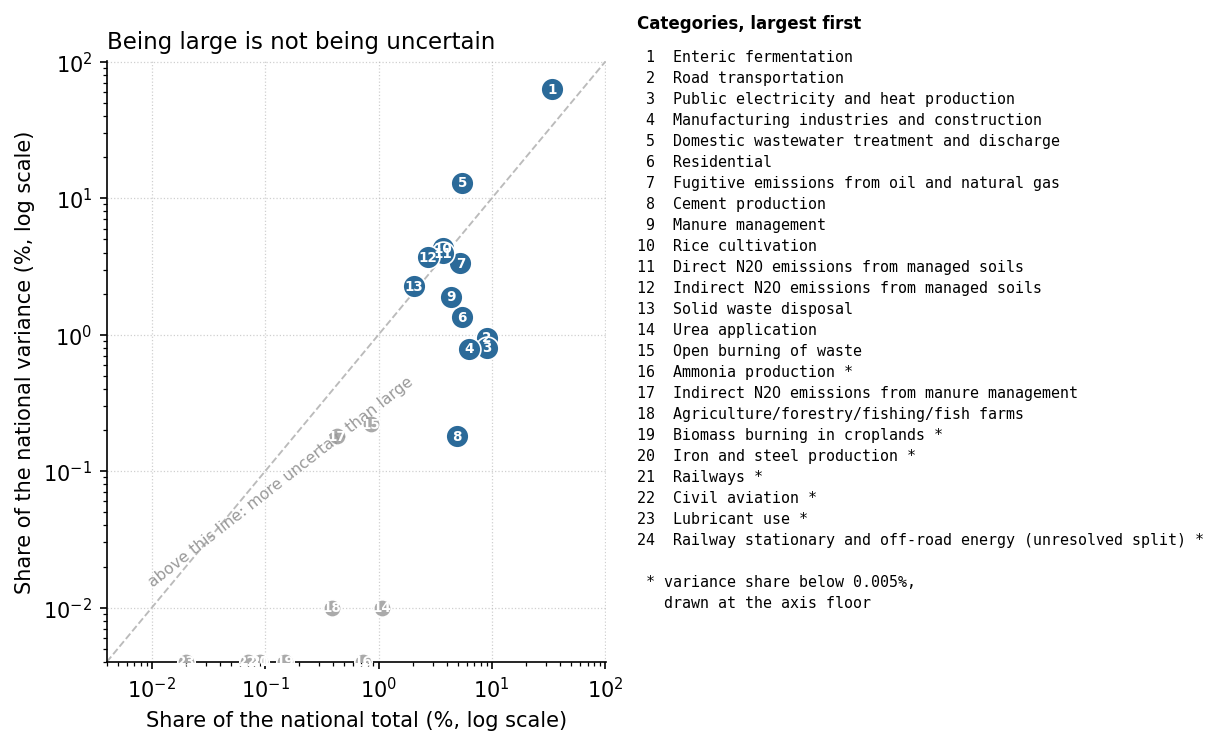
\includegraphics[width=\linewidth]{national_key_categories.png}
\caption{Level share against variance share for all \num{24} IPCC categories, on
\textbf{log axes}. The diagonal still marks equal level and variance share, so the reading is
unchanged: above it a category contributes more to national uncertainty than to magnitude. A
previous edition drew this linearly, which put enteric fermentation at one corner and
compressed eleven categories into a blot at the other---and the low corner is where the
finding is.}
\label{fig:keycat}
\end{figure}

\subsection{What the two rankings imply}

\textbf{Road transport} contributes \SI{9.0}{\percent} of emissions but
\SI{0.9}{\percent} of variance. Its fuel control and carbon factor constrain national mass,
so more fleet detail would improve composition and air-pollutant analysis more than the
national greenhouse-gas interval.

\textbf{Domestic wastewater} contributes \SI{5.5}{\percent} of emissions and
\SI{13.0}{\percent} of variance. It is the largest upward inversion after enteric
fermentation, and its uncertainty has two named drivers: the
methane correction factor for Pakistani sewers, now the larger term, and the
effluent N$_2$O factor's bounded 150-fold published range, which the 2019 Refinement
shortened from the 2006 Guidelines' 500-fold. Dissolved-methane sampling on urban drains
and an effluent-pathway N$_2$O measurement would test the two directly, in that order.

\textbf{Oil and gas fugitives} are now key by level. The completed 2019 segment account is
\SI{5.3}{\percent} of emissions and \SI{3.3}{\percent} of Approach-1 variance. This replaces
the earlier production-only result in which a very small category carried a four-order-of-
magnitude factor range. The remaining priority is no longer simply utility throughput: it is
technology and facility evidence for pipeline material, pressure, LDAR, compressors,
processing and wells.

\textbf{Enteric fermentation} remains dominant on both rankings, at
\SI{34.1}{\percent} of emissions and \SI{63.0}{\percent} of variance. The variance ranking
therefore supports work on both livestock and wastewater; it does not imply that one small
category alone controls national uncertainty.

\subsection{The ten-sector trend, and what its window can and cannot say}

IPCC's trend assessment requires a consistent series between one base and reference year.
All ten sectors now satisfy that requirement from FY2016--17 onward and are published as
the constant-scope view (Section~\ref{sec:series}), so the \emph{ten-sector} trend this
release previously declared out of reach is the one it supports. Cement and industrial
combustion were the two holding it back; both were absent for want of documents that turned
out to be held, and both now report every year of the window. The window now reaches
FY2015--16 as well: the product splits that blocked transport and industry there were
recovered from the publicly served Pakistan Oil Report 2015--2016 under a four-way identity
gate, so the full nine-year panel is a like-for-like base for the trend. The agriculture-only trend assessment carries a heavier qualification than
the others and it should be read with it: crop and nitrogen activity is now reconstructed on
Pakistani fiscal-year tables in every year, but enteric fermentation and manure management
still ride a calendar-year livestock projection because no fiscal enumeration of the herd
exists, so the sector's history is fiscal in the categories that could be moved and a
declared calendar projection in the \SI{77.37}{\percent} that could not
(Section~\ref{sec:agri-basis}).

\pkinvEndFragment


\section{Usage notes and limitations}\label{sec:usage}
Fitness for use depends on species, process, period, configuration and evidence support. Covered totals, conditional percentiles, structural cases, provisional sources and missing categories are distinct products. Administrative/cell allocations and monthly proxies must not be read as observed local emissions or atmospheric concentration.
\pkinvLeadFragment
\section{Limitations and fitness for use}
\label{sec:limitations}
\subsection{Scope, period and source support}
\label{lim:single-year}\label{lim:series-basis}\label{lim:incomplete-floor}
The common core spans ten fiscal years, July 2015--June 2025. It is not a full calendar-year 2015--2025 series. FY2023--24 remains the detailed reference uncertainty/spatial year because source support and latest annual availability answer different questions. FY2025--26 source/sector extensions are provisional and separate; their partial sums are not common-scope national totals.

A complete ten-module/year rectangle is compatible with substantial missing source categories. Native GHG and air products describe admitted sources under named configurations. External differences are not inventories of missing mass, and no unrelated global emissions are silently added. F-gases, coal-mining fugitives and remaining industrial/treatment sources retain explicit coverage records.

\label{lim:lulucf}
The scope is non-LULUCF. Exploratory land-sector estimates remain outside totals and are not treated as a validated correction to the national inventory. An omitted land flux may be a sink or source and cannot be interpreted as a one-direction bias.

\subsection{Shared accounting and structural choices}
\label{lim:soft-partitions}\label{lim:firewood}
Station coal consumption and rank-specific NCV define the power reference. Supply, receipts, stock change, consumer bookings and generation are distinct observations. Residual coal is explicitly unresolved where supported consumer evidence cannot allocate it; independently uncertain records do not become an exact physical balance merely because a published table is constructed as a residual identity. Dated kiln-fleet operating cases test credible alternatives without pretending to be an observed annual series or assigning them probabilities.

Household S uses survey dung and wood quantities, with historical interpolation or extrapolation labelled. L assumes all ledger-diverted dung is burned in households. The unobserved destination of remaining diverted dung is not resolved by material conservation. Survey recall, stove/fuel transfer factors and geographic proxies remain consequential uncertainty.

\label{lim:fugitive-envelope}
Fugitive methane remains conditional on practice, factor applicability and source coverage. Unaccounted-for gas includes non-leak components and is not equated to methane leakage. Native bounded source/fate draws are used where supported. Flaring and venting are distinct; their activity cannot be counted again in energy or IPPU.

\subsection{Air methods and uncertainty}
\label{lim:air-pollutants}\label{lim:tier1}
Air emissions use common activity but pollutant-specific factors, controls and chemical mass conventions. The seven core species have source--process coverage cells; industry, IPPU and fugitives include admitted provisional estimates. Power oil/diesel SO$_2$ is admitted separately from coal/gas/bagasse scenarios. Port Qasim and China Power Hub licences describe proposed design controls; installed or continuously operating removal is not demonstrated. Screening endpoints are typical-factor scenarios, not mathematical upper bounds.

Road methods include hot/cold exhaust, evaporation and tyre/brake/surface wear; resuspended dust and off-road air estimates remain absent. Transferred fleet-average factors, vehicle-age/technology composition, CNG-to-LPG chemistry and petrol-bus substitutions remain documented proxies. A valid fuel/CO$_2$ balance does not validate NO$_x$ or particulate factors. Fuel-sulfur policy dates are specification evidence, not universal pump-level measurements.

Residential results are gross appliance releases. An outdoor escape fraction, vertical injection, detailed chemical speciation and atmospheric transport are not supplied. Waste burning geography follows origin rather than observed disposal/fire sites. Emissions rankings do not measure concentration, exposure or health-intervention priority. BC/OC and particulate strata are non-additive.

The TAN reference conserves stage-resolved nitrogen across NH$_3$, NO$_x$ and N$_2$O; IPCC is a separate regenerated configuration. Conditional parameter ensembles share actual herd, crop, nutrient, waste and fugitive inputs and retain bounded fractions. Paired years produce trend intervals. Management shares, excretion, control operation, structural factor alternatives, missing categories and allocation uncertainty remain outside these percentiles. Dry-climate soil-factor applicability is evaluated separately for irrigated cropland, rice and grazing; matching FAOSTAT does not select a factor.

\subsection{Timing and location}
\label{lim:monthly-physics}\label{lim:monthly-grade}\label{lim:monthly-gap}
Monthly availability is assessed from the final exported activity, geographic coverage and compatible source controls. PDF group labels, continuation rows and worksheet identity are preserved when the PBS tables are read. Source anomalies that survive correct transcription remain flagged and an unsupported national profile is replaced by a declared weaker fallback. Twelve months alone never establish national observed activity.

Fertiliser offtake is a supply-timing proxy. Manure-stage, residue-decomposition, waste burning and unsupported evaporation/wear seasonality use declared fallback allocation. A CO$_2$-equivalent-weighted timing score does not describe an air pollutant; temporal and spatial evidence shares are calculated separately by species.

Grid cells carry allocated mass, not observed activity at 0.05$^\circ$. Fixed reference-year proxies do not establish changing local geography. Facilities respect commissioning/closure windows. Placed plus unallocated mass is conserved, and territories/country masks retain their stated boundaries. Cell mass differs from flux density; area, country fraction and period duration are required for conversion.

\subsection{Evaluation and availability}
\label{lim:deposit}
Matched comparisons separate magnitude, change, timing and location and record shared inputs. HTAPv3.2's direct country/monthly bundles are publicly available without credentials; a restricted optional spatial-subset service is not a restriction on those files. REAS/EDGAR inputs and EDGAR trend extensions limit independence. Satellite columns require chemistry, transport, retrieval and sampling treatment before they constrain emissions; a simple concentration--emission correlation is insufficient.

The review package contains current products, metadata, code, reproduction instructions and licences/checksums. Product-level licences distinguish independently sourced primary geography from ODbL-derived alternatives. A local package is not an external archive deposit, and no DOI or journal submission is asserted until that separately authorised action occurs.

\pkinvEndFragment
\pkinvDemoteFragment
% ===========================================================================
\section{Discussion}
\label{sec:discussion}
% ===========================================================================

\subsection{What the architecture actually bought}

The claim in Section~\ref{sec:architecture} is testable against the project's own history,
and it is worth being honest about which parts of it paid off.

The clearest return was on \emph{late additions}. Fugitives and cement were built last, after
the analysis layer was mature. Neither required any change to the uncertainty analysis, the
key-category screen, the benchmark comparison, the provincial allocation or the figure
generation; both appeared in every national output on first registration. In a spreadsheet
inventory, adding a sector means extending every downstream sheet by hand, and the cost of a
new sector rises with the number of sectors already present. Here it is flat.

The second return was on \emph{invariants catching real errors}. Several of the \num{27}
contract tests exist because they failed, and Table~\ref{tab:qa} is the audit rather than the
anecdote: each row is a defect this project shipped, what it would have cost, how it was
found, and the guard that now makes it a build failure. The pattern across them is worth more
than any single row. \textbf{Every one was invisible to review}, because nothing about the
resulting numbers looked wrong---and the later ones were invisible to the numeric tests too,
because they were claims about words, boundaries or layout rather than about digits.

\begin{table*}[htbp]
\centering
\footnotesize
\setlength{\tabcolsep}{4pt}
\begin{tabular}{@{}p{0.19\linewidth}p{0.17\linewidth}p{0.16\linewidth}p{0.18\linewidth}p{0.20\linewidth}@{}}
\toprule
\textbf{Defect} & \textbf{Consequence} & \textbf{Detection} & \textbf{Correction} &
\textbf{Regression guard} \\
\midrule
Two sectors proposing one category name & silent double-count & contract test on
registration & globally unique names & category-name invariant \\
Correlation group spanning two categories & variance apportionment ill-defined & contract
test & groups within one category & correlation-group invariant \\
Wrong parallel factor table & category trace gases 8\% out, \COtwo{} exact & factor audit &
category-specific factor identity & factor-identity test \\
Ambiguous integer year labels & mixed-period national total & period audit & explicit
start/end dates & period-schema test \\
Unread public activity table & \SI{3.40}{\mega\tonne} coverage gap & repository audit & OCAC
liquid customer class read & completeness test \\
Retired provincial power proxy & \SI{8.8}{\mega\tonne} in the wrong province & spatial
diagnostic & plant-wise generation & allocation test \\
Source documents never archived & provenance unverifiable & archive audit & source-document
registry & document-manifest test \\
Figure sources named by year & two manuscripts shipped pre-harmonisation figures & external
review & year resolved at read time, absence raises & figure-source test \\
Stale gas decomposition & a decomposition summing to \SI{455.14}{\mega\tonne} against a
printed \SI{448.00}{} & external review & generated category~$\times$~gas ledger &
gas-total invariant \\
Declared-debt list & printed quantities tracked but unverified & external review & the list
deleted; no exemption without a reason & unconditional coverage test \\
Two category hierarchies & \num{20} categories screened against \num{24} reported & external
review & IPCC category made canonical & one-hierarchy test \\
Stale comparative language & ``doubles'' surviving a ratio of \num{1.61} & external review &
claims registry binding phrase to relation & semantic-claims test \\
One correlation group per row & a factor correlation reported as widening a category by more
than half when it moves it by nothing & external review & uncertainty carried per parameter &
decomposition-identity test \\
Content printed off the page & \SI{104}{pt} of a table outside the margin & external review &
tables narrowed & log-derived layout test \\
\addlinespace
Superseded output vintage & a retired FY2019--20 fugitives file quoting
\SI{3.81}{\mega\tonne} beside the then-current \SI{24.69}{} (the envelope's top) & rebuild
audit & vintage retired &
orphan and twin sweep over \texttt{outputs/} \\
Staleness guard reading it & the shipped-versus-engine check ran on three sectors of nine and
reported passing & rebuild audit & the check reads each sector's declared categories &
per-sector coverage asserted, not assumed \\
Orchestrator declaring outputs it did not write & four phases named files that existed
nowhere and printed OK beside them & rebuild audit & the declared artefact must be written
during the run & orchestrator output check \\
Run manifest listing a directory scrape & a sector's manifest claimed any leftover file as
its own product & rebuild audit & the manifest records what the run wrote & write-tracked
manifest \\
The build defined three times & the branch that gates merges built a smaller inventory than
either local command & rebuild audit & the three lists reconciled & build-definition test \\
The release record & it printed \SI{455.14}{\mega\tonne} and described a mixed-year
inventory three rounds after both stopped being true & rebuild audit & repaired and anchored
& the release record is a claims document \\
\bottomrule
\end{tabular}
\caption{Defects this inventory shipped, and what now prevents each. The right-hand column is
the deliverable: a defect without a regression guard has been corrected, not closed. The
detection column is the uncomfortable one---the middle entries were found by an external
reader rather than by the suite, and each of those had passed a suite of more than a thousand
tests, because the property that was wrong had never been made checkable. The last six were
found by rebuilding the whole release from one commit and asking a narrower question than the
suite asks: not whether each artefact is correct, but whether anything still writes it. Four
of the six are the same defect wearing different clothes---a check that reports passing while
testing nothing---which is the failure mode a growing test suite is least able to see in
itself.}
\label{tab:qa}
\end{table*}

The third, and least anticipated, was that \emph{closures turned prose caveats into
arithmetic}. The four enforced closures in Section~\ref{sec:closures} existed first as written
warnings---``this biases the sector high'', ``there is no national figure to remove them
by''---in the documentation of sectors that had done the honest thing and declared a known
defect. Building the counterpart sector converted each warning into a number. That is a
general pattern worth naming: a well-documented known defect is a specification for the work
that fixes it.

What the architecture did \emph{not} buy is accuracy. The engine's activity data are still
national statistics of variable quality, its factors are still mostly IPCC Tier~1 defaults,
and the largest sector rests on a livestock census. Structure prevents inconsistency; it does
not manufacture information.

\subsection{Two undeclared assumptions worth a table apiece}

Two results in this paper share a shape, and the shape is the point.

Sharing parameters by physical identity across modules, rather than confining them within
one, leaves the national uncertainty at $\pm\SI{11.72}{\percent}$ and the
road-transport category unmoved---a result that reverses
what the previous edition reported, for reasons Section~\ref{sec:uncertainty} sets out. The sewer methane correction factor
moves domestic wastewater from \SI{15.39}{\mega\tonne} to \SI{24.46}{\mega\tonne}---a factor of \num{1.6} on a category that is \SI{5.5}{\percent} of the national inventory. In both
cases the assumption is defensible in either direction, the evidence does not settle it, and
the conventional treatment is to pick one and not mention it.

We publish both endpoints in both cases. That is not fence-sitting; it is the recognition
that a single number carries a false claim about the state of knowledge, and that the correct
output of an analysis whose answer depends on an unsettled assumption is the dependence
itself. In both cases we also state what would settle it: for correlation, a Pakistani fuel
carbon-content measurement programme; for the MCF, dissolved-methane sampling on urban drains
in two or three cities.

\subsection{Implications for Pakistani inventory work}

Three practical conclusions follow, in descending order of confidence.

\textbf{Resolve gas-system practices before refining the vehicle fleet.} The 2019 segment
ledger now includes utility throughput and pipeline length, making fugitives
\SI{5.3}{\percent} of national emissions and \SI{3.3}{\percent} of variance. Road transport
is \SI{9.0}{\percent} and \SI{0.9}{\percent}. The binding fugitive evidence is therefore
pipeline material and pressure, LDAR, compressor configuration, processing throughput and
well status rather than another aggregate production factor.

\textbf{Industrial fuel combustion is the binding constraint on completeness.} At roughly
\SI{16}{\mega\tonne} still missing, the unestimated remainder alone would rank sixth among
this inventory's modules---just below residential fuel---while the complete \SI{43.98}{\mega\tonne}
category EDGAR reports would rank third, above road transport. Its absence is
most of why this inventory reports \SI{87}{\percent} of EDGAR's aggregate magnitude. No amount of
refinement elsewhere compensates for the unmeasured fuels within this partially estimated
industrial category.

\textbf{Methane is the metric-sensitive majority.} At \SI{54.6}{\percent} of the national
total on AR5, Pakistan's inventory is dominated by a short-lived gas, and mitigation
assessments will be unusually sensitive to the metric and time horizon chosen. Reporting both
AR5 and AR6 at every level of aggregation, as here, is a minimum; a country in this position
has a stronger case than most for also reporting on a short-horizon metric.

\subsection{Co-emitted air pollutants: a companion product, not a result of this paper}

Seven of the ten modules also compute an air-pollutant layer from the same activity
quantities, through EMEP/EEA factors \citep{emep2019,emep2023soils} rather than from a
separate study. That shared activity basis is the methodologically interesting part, and it
supports one robust statement: on primary \PM{}, household solid fuel is the largest estimated
source in this inventory by a wide margin, while being a minor greenhouse-gas category---the
two inventories rank sources close to inversely.

\textbf{It is reported in the supplement rather than here, deliberately.} The seven layers are
not of comparable assurance: two are bounds or screening estimates, transport is exhaust-only,
and industrial combustion and IPPU have no layer at all. A ranking drawn across evidence that
uneven is easy to over-read, and it should not carry weight the greenhouse-gas product has
earned and it has not. Supplementary Note~S1 gives the layer-by-layer assurance matrix, the
magnitudes and the figure, released as \textbf{PakEmis-Air beta}.

\subsection{Generalisability}

The architecture is not Pakistan-specific. The contract in Section~\ref{sec:architecture}
encodes properties of IPCC inventories generally---categories, gases, notation keys,
allocation proxies, correlation groups---and the accounting closures are instances of a
pattern (one national quantity consumed by two sectors) that recurs in every national
inventory: refinery fuel between 1A1b and 1A2, waste between disposal and incineration, land
between cropland and grassland.

The parallel-table trap of Section~\ref{sec:factors} is entirely general and, we would
expect, common. Any inventory compiled by a small team under time pressure, using the 2006
Guidelines, is exposed to it, and the exposure is invisible to \COtwo{}-based validation.
Checking which of the four Chapter~2 tables and which of the Chapter~3 tables each fuel-using
category actually drew from would be a cheap and, we suspect, productive audit of many
published national inventories.

\pkinvEndFragment



% ---------------------------------------------------------------------------
% 8 Conclusions
% ---------------------------------------------------------------------------
\conclusions
\label{sec:essd-conclusions}
\pkinvLeadFragment
\section{Conclusions}\label{sec:conclusion}
PakEmis \PakEmisRelease\ supplies one non-LULUCF greenhouse-gas and air-pollutant reconstruction for Pakistan over July 2015--June 2025. Native species and separate GWP metrics, source-process coverage, four integrated configurations, annual/monthly and geographic products, conditional uncertainty and source cases describe the same inventory account.

Station consumption/rank coal, reconciled consumer residuals, survey-supported household activity and conserved nitrogen pathways are consequential scientific changes. Supported FY2026 sources extend information provisionally without becoming a full national year. Public HTAP/EDGAR comparisons and source/export checks expose differences and limits rather than tuning estimates to agreement. Further improvement depends on source activity, management, factor applicability and demonstrated control evidence; nominal grid resolution alone cannot resolve those gaps.

All essential local review assets are prepared or identified by the release manifest and product-specific licensing record. A public repository review deposit and persistent dataset identifier remain separate external actions, with no submission or acceptance claim implied by this technical report.

\pkinvEndFragment

% ---------------------------------------------------------------------------
% Data availability and Code availability: GENERATED from the release manifest.
% ---------------------------------------------------------------------------
%% GENERATED by scripts/make_availability.py from outputs/release_manifest.json.
%% Do not edit: the edit will be overwritten and a test compares this file to a fresh render.
\dataavailability{The dataset described here is PakEmis 1.0.0rc67. The dataset DOI is assigned on deposit; until then the release is identified by version and manifest digest (\texttt{outputs/release\_manifest.json}, whose SHA-256 the release cover of every technical note prints).
The technical documentation---the sector technical notes and this supplement---is deposited with the data under the documentation record, whose identifier is assigned with the dataset's.
The manifest records the licences as MIT for the code and CC-BY-4.0 for the data and text, with the OpenStreetMap-derived carve-outs it lists under ODbL~1.0.
One evaluation-only input carries no licence declaration in the record and is excluded from the primary data record until its rights are established (the manifest's \texttt{licences.undetermined} note).
\ifdefined\pkinvDataTerms\pkinvDataTerms\fi}

\codeavailability{The software is release 1.0.0rc67 of the \texttt{pkinv} package (manifest schema \texttt{pkinv.release/v1}). The software DOI is assigned on deposit, with the dataset's; until then the release is identified by version and manifest digest.
\ifdefined\pkinvCodeTerms\pkinvCodeTerms\fi}


\authorcontribution{RA designed the inventory system, acquired and transcribed the source
documents, wrote the engine and its tests, produced the data records and wrote the paper.}

\competinginterests{The author declares no competing interests.}

\bibliographystyle{copernicus}
\bibliography{../../../paper_common/references}

\end{document}
